% !TEX root = ../notes_template.tex
\chapter{Vectors}\label{chp:vectors}

% \minitoc

\section{$n$-Vectors}
A collection of an ordered list of $n$ numbers is called an $n$-vector. We will use bold lowercase alphabets to represent such vectors, and we will represent these as a column of numbers, which is referred to as a \textit{column vector}. We will look at \textit{row vectors} at a later stage. Consider the following example:
\[ \mf{x} = \bmxc x_1 \\ x_2 \\ \vdots \\x_n \emx \]

The elements of the $n$-vector $x_1, x_2, \ldots, x_n$ are called the \textit{components} of the vector $\mf{x}$; $x_i$ is the $i^{th}$ component of the vector $\mf{x}$. If these components are all real numbers, the set of all such $n$-vectors is the set $\mb{R}^n$.

\noindent \textbf{Where do we come across such $n$-vectors?} In many places, such as in physics, engineering, economics, medicine, etc. Any application where we deal with multiple pieces of information that can be represented as a list of numbers can be represented as an $n$-vector. When we deal with systems with multiple inputs, multiple outputs, or multiple states, we can represent these as $n$-vectors. We talk about the state of a system in a later chapter.

\subsection{Some common $n$-vectors}
We will often come across some special $n$-vectors in this document course and in many applications. We will define some of these vectors here.
\begin{itemize}
    \item \textbf{Zero vector:} The $n$-vector whose components are all zeros is called the \textit{zero vector}. $\mf{0} = \bmxc 0 \\ 0 \\ \vdots \\ 0\emx$
    \item \textbf{One vector:} The $n$-vector whose components are all ones is called the \textit{one vector}. $\mf{1} = \bmxc 1 \\ 1 \\ \vdots \\ 1\emx$
    \item \textbf{Unit vectors:} The $n$-vectors whose components are all zeros except for one component, which is 1. These are called the \textit{standard basis vectors} and are denoted by $\mf{e}_1, \mf{e}_2, \ldots, \mf{e}_n$. The $n$-vector $\mf{e}_i$ has all components as zeros except for the $i^{th}$ component, which is 1. For example, the unit vectors in $\mb{R}^2$ are:
    \[ \mf{e}_1 = \bmx 1 \\ 0\emx \quad \mf{e}_2 = \bmx 0 \\ 1 \emx  \]
\end{itemize}

We now look at some examples of $n$-vectors that we come across in applications.

\begin{boxedstuff}
    \begin{example}
        \textbf{Basic clinical information during a hospital visit}. When a patient visits a hospital, several clinically relevant variables are captured, for instance:
        \begin{small}
            \begin{center}
            \begin{tabular}{ccc}
                \hline
                \textbf{Index} & \textbf{Variable} & \textbf{Units} \\ \hline
                1 & Sex & None (0: Male, 1: Female) \\
                2 & Age & Years \\
                3 & Height & cm \\
                4 & Weight & kg \\
                5 & Heart rate & count \\
                6 & Systolic pressure & mm of Hg \\
                7 & Diastolic pressure & mm of Hg \\
                8 & Temperature & celcius \\ \hline
            \end{tabular}
            \end{center}
        \end{small}
        The following are some examples of $n$-vectors generated from three different patients visiting the hospital.
        \begin{equation*}
            \mf{x}_1 = \bmxc 1 \\ 67 \\ 152 \\ 56 \\ 132 \\ 102 \\ 37.1 \emx \quad \mf{x}_2 = \bmxc 0 \\ 36 \\ 172 \\ 97 \\ 156 \\ 97 \\ 36.5 \emx \quad \mf{x}_3 = \bmxc 1 \\ 22 \\ 162 \\ 56 \\ 121 \\ 78 \\ 38.2 \emx
        \end{equation*}
    \end{example}

    \begin{example}
        \textbf{Time series data}. We often collect data over time, often at regular intervals. For example, consider the example of an attending nurse taking the temperature of a patient admitted to the hospital for an infectious disease. The nurse records the temperature of the patient every hour, without fail, for the 48 hours the patient spent in the hospital. This temperature record will have a total of 49 measurements, which can conveniently be thought of as a $n$-vector, in this case, a $49$-vector. Instead of writing down the entire $49$-vector, we depict it as a time series plot.
        \begin{center}
            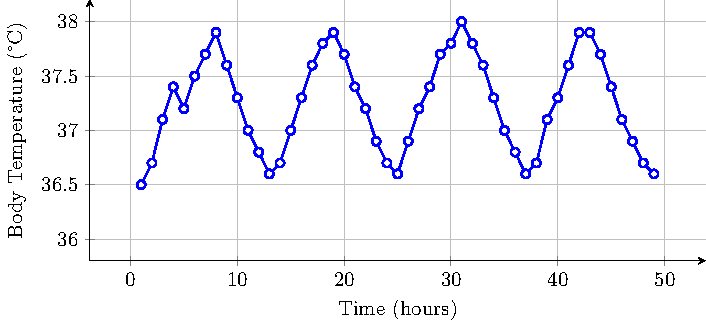
\includegraphics[width=0.5\textwidth]{figure/chapter01/temp-ts.pdf}
            \captionof{figure}{Body temperature recorded at multiple time points.}
        \end{center}
    \end{example}
\end{boxedstuff}

\section{Visualizing $n$-vectors}
The $n$-vectors can be visualized as points in $n$-dimensional space. For example, A 1-vector or just a single real number or a \textit{scalar} can be thought of as a point on the real line. The 1-vector $x = 2.45$ is shown in Figure~\ref{fig:ch01-1-vector} is the black point. But we will find it useful to visualize a 1-vector as an arrow starting at the origin and ending at the point on the real line. The arrow is shown in blue in Figure~\ref{fig:ch01-1-vector}. 

\begin{figure}[b]
    \centering
    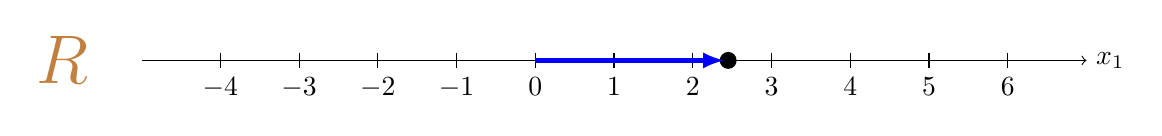
\begin{tikzpicture}
        \draw[->] (-5,0) -- (7,0) node[right] {$x_1$};
        \foreach \x in {,-4,-3,-2,0,-1,1,2,3,4,5,6}
            \draw (\x,0.1) -- (\x,-0.1) node[below] {$\x$};
        % Plot an example point and its corresponding arrow
        \draw[fill=black] (2.45,0) circle (0.1); % Smaller marker size
        \draw[-latex, ultra thick, blue] (0,0) -- (2.4,0); % Thicker arrow
        % Huge font for the label with brown color
        \node[font=\Huge, text=brown] at (-6, 0) {$\mathbb{R}$};
    \end{tikzpicture}
    \caption{The real line $\mb{R}$ contains the $1$-vectors.}
    \label{fig:ch01-1-vector}
\end{figure}

The elements of $\mb{R}^2$ are points on the plane, and we can visualize them as points in the plane. The 2-vectors $\mf{x} = \bmxc 2 \\ 3 \emx$ and $\mf{x} = \bmxc -3 \\ 1 \emx$ are shown in Figure~\ref{fig:ch01-2-vector}. A similar visualization is shown for $\mb{R}^3$ (Figure~\ref{fig:ch01-3-vector}), and for $\mb{R}^4$ and beyond, you simply pretend that you can visualize things in your head like your instructor does.

\begin{figure}[t]
    \centering
    \begin{subfigure}[b]{0.45\textwidth}
        \centering
        \begin{tikzpicture}[scale=0.6]
            \draw[->, gray] (-5,0) -- (5,0) node[right] {$x_1$};
            \draw[->, gray] (0,-5) -- (0,5) node[above] {$x_2$};
            \foreach \x in {-4,-2,-1,2,4}
            \draw (\x,0.1) -- (\x,-0.1) node[below, gray] {$\x$};
            \foreach \y in {-4,-2,-1,2,4}
            \draw (0.1,\y) -- (-0.1,\y) node[left, gray] {$\y$};
            % Plot an example point and its corresponding arrow
            \draw[fill=black] (2,3) circle (0.1); % Marker for the point (2,3)
            \draw[-latex, ultra thick, blue] (0,0) --  (2,3) node[right, black] {$\mathbf{x} = \begin{bmatrix} 2 \\ 3 \end{bmatrix}$}; % Arrow with label
            
            \draw[fill=black] (-3,1) circle (0.1); % Marker for the point (-2,1)
            \draw[-latex, ultra thick, red] (0,0) --  (-3,1) node[left, black] {$\mathbf{y} = \begin{bmatrix} -3 \\ 1 \end{bmatrix}$}; % Arrow with label
            
            % Huge font for the label with brown color
            \node[font=\Huge, text=brown] at (-4, 4) {$\mathbb{R}^2$};
        \end{tikzpicture}
        \caption{The $\mathbb{R}^2$ plane contains the $2$-vectors.}
        \label{fig:ch01-2-vector}
    \end{subfigure}
    \begin{subfigure}[b]{0.45\textwidth}
        \centering
        \tdplotsetmaincoords{60}{120} % Set the view angle
        \begin{tikzpicture}[scale=0.7,tdplot_main_coords] % Set scale and use the main coordinates
            % Axis lines
            \draw[->, gray] (-5,0,0) -- (5,0,0) node[anchor=north east]{$x_1$};
            \draw[->, gray] (0,-5,0) -- (0,5,0) node[anchor=north west]{$x_2$};
            \draw[->, gray] (0,0,-5) -- (0,0,5) node[anchor=south]{$x_3$};
            \foreach \x in {-4,-2,,2,4}
                \draw (\x,0,0.1) -- (\x,0,-0.1) node[below, gray] {$\x$};
            \foreach \y in {-4,-2,,2,4}
                \draw (0.1,\y,0) -- (-0.1,\y,0) node[above right, gray] {$\y$};
            \foreach \z in {-4,-2,,2,4}
                \draw (0.1,0,\z) -- (-0.1,0,\z) node[above right, gray] {$\z$};
            % Points
            \draw[fill=blue] (1,2,3) circle (0.08);
            \draw[-latex, ultra thick, blue] (0,0,0) --  (1,2,3) node[above, black] {$\mathbf{x} = \bmx 1 \\ 2 \\ 1 \emx$}; 
            % Points
            \draw[fill=red] (2,-1,1) circle (0.08);
            \draw[-latex, ultra thick, red] (0,0,0) --  (2,-1,1) node[below left, black] {$\mathbf{y} = \bmx 2 \\ -1 \\ 1 \emx$}; 
             
            % Huge font for the label with brown color
            \node[font=\Huge, text=brown] at (2,-2,4.5) {$\mathbb{R}^3$};
        \end{tikzpicture}
        \caption{$\mb{R}^3$ contains the 3-vectors.}
        \label{fig:ch01-3-vector}
    \end{subfigure}
    \caption{The $\mb{R}^2$ and $\mb{R}^3$ sets.}
    \label{fig:ch01-combined}
\end{figure}

\section{Operations on $n$-vectors}
There are many operations we can perform on $n$-vectors, but we will only focus on two operations for this course:
\begin{itemize}
    \item \textbf{Scalar multiplication:} Given a scalar $c \in \mb{R}$ and an $n$-vector $\mf{x}$. The scalar multiplication operation produces another $n$-vector $c\mf{x}$ whose components are $cx_1, cx_2, \ldots, cx_n$. 
    \[ \mf{x} = \bmx 1 \\ 2\emx \longrightarrow 2 \mf{x} = \bmx  2\ct{1} \\ 2\ct{2} \emx = \bmx  2 \\ 4 \emx \]

    The geometric interpretation of scalar multiplication is shown in Figure~\ref{fig:ch01-scalar-mult}. Scalar multiplication stretches or shrinks the vector without rotating it. When the scalar is positive, the direction of the scaled vector is the same as the original vector, and when the scalar is negative, the direction is opposite. When the scalar is zero, the scaled vector is the zero vector $\mf{0}$. 
    \begin{figure}[h!]
        \centering
        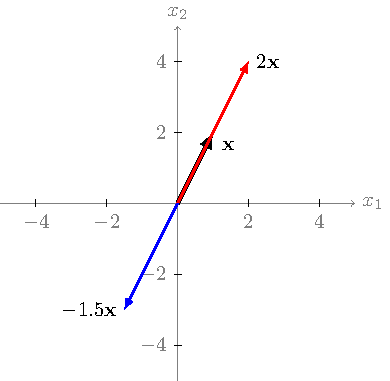
\includegraphics{figure/chapter01/vec-scale.pdf}
        \caption{Scalar multiplication of a vector.}
        \label{fig:ch01-scalar-mult}
    \end{figure}
    
    \item \textbf{Vector Addition:} Given two $n$-vectors $\mf{x}$ and $\mf{y}$, the vector addition operation, represented by $\mf{x} + \mf{y}$, produces another $n$-vector whose components are $x_1 + y_1, x_2 + y_2, \ldots, x_n + y_n$.
    \[ \mf{x} = \bmxc 1 \\ 3 \emx, \mf{y} = \bmxc 2 \\ 1 \emx \longrightarrow \mf{x} + \mf{y} = \bmxc 1 + 2 \\ 3 + 1 \emx = \bmxc 3 \\ 4 \emx \]
    
    \begin{figure}[h!]
        \centering
        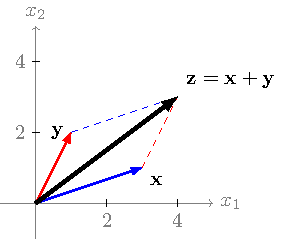
\includegraphics{figure/chapter01/vec-add-fig.pdf}
        \caption{Vector addition.}
        \label{fig:ch01-vec-add}
    \end{figure}

    The geometric interpretation of the vector addition operation is shown in Figure~\ref{fig:ch01-vec-add}. Geometrically, the vector addition operation follows the parallelogram law of addition, where the resulting vector $\mf{x} + \mf{y}$ is a diagonal of the parallelogram formed by the two vectors $\mf{x}$ and $\mf{y}$. Another way to think about this is that you first move along $\mf{x}$ to its endpoint, and starting from there, then move along $\mf{y}$ to its endpoint or vice versa.

    You can add more than two vectors to obtain a new vector, like below:
    \[ \mf{w} = \mf{x} + \mf{y} + \mf{z} \]
    Geometrically, we can first apply the parallelogram law to $\mf{x}$ and $\mf{y}$, and then apply the parallelogram law to $\mf{x} + \mf{y}$ and $\mf{z}$ to get $\mf{w}$.
\end{itemize}


\section{Vector spaces}
Vector spaces are \textit{sets} with some special properties. More specifically, a vector space is a set $V$ of elements called \textit{vectors} that are closed under two operations called \textit{addition} and \textit{scalar multiplication}. This simply means that if you perform these operations using elements from the set $V$, the result is also an element of the set $V$. A vector space must satisfy the following properties:
\begin{itemize}
    \item \textbf{Closure under addition:} For any two vectors $\mf{x}, \mf{y} \in V$, the sum $\mf{x} + \mf{y} \in V$.
    \item \textbf{Closure under scalar multiplication:} For any scalar $c \in \mb{R}$ and any vector $\mf{x} \in V$, the product $c\mf{x} \in V$.
    \item \textbf{Additive identity:} There exists a vector $\mf{0} \in V$ such that for any vector $\mf{x} \in V$, $\mf{x} + \mf{0} = \mf{x}$.
    \item \textbf{Additive inverse:} For any vector $\mf{x} \in V$, there exists a vector $-\mf{x} \in V$ such that $\mf{x} + (-\mf{x}) = \mf{0}$.
    \item \textbf{Commutativity of addition:} For any two vectors $\mf{x}, \mf{y} \in V$, $\mf{x} + \mf{y} = \mf{y} + \mf{x}$.
    \item \textbf{Associativity of addition:} For any three vectors $\mf{x}, \mf{y}, \mf{z} \in V$, $(\mf{x} + \mf{y}) + \mf{z} = \mf{x} + (\mf{y} + \mf{z})$.
    \item \textbf{Distributive property:} For any scalar $c \in \mb{R}$ and any two vectors $\mf{x}, \mf{y} \in V$, $c(\mf{x} + \mf{y}) = c\mf{x} + c\mf{y}$.
    \item \textbf{Distributive property:} For any two scalars $c, d \in \mb{R}$ and any vector $\mf{x} \in V$, $(c + d)\mf{x} = c\mf{x} + d\mf{x}$.
    \item \textbf{Associativity of scalar multiplication:} For any two scalars $c, d \in \mb{R}$ and any vector $\mf{x} \in V$, $(cd)\mf{x} = c(d\mf{x})$.
    \item \textbf{Multiplicative identity:} For any vector $\mf{x} \in V$, $1\mf{x} = \mf{x}$.
\end{itemize}
These properties are satisfied by the set $\mb{R}^n$ of $n$-vectors, and hence $\mb{R}^n$ is a vector space. Geometrically, the concept of a vector space corresponds to flat spaces that contain the origin. This will become more clear when we talk about subspaces. Notice that the definition of the vector space given above does not make any specific mention of $n$-vectors. The definition is general and can be applied to any set of elements that satisfy the properties listed above. The following are some examples of vector spaces with the addition and scalar multiplication operations defined on them.

\begin{boxedstuff}
\begin{example}
    \textbf{Set of $m \times n$ matrices.} The set $M$ of all $m \times n$ matrices of real numbers is a vector space.
    \[ \mf{A} = \bmxc
        a_{11} & a_{12} & \cdots & a_{1n} \\
        a_{21} & a_{22} & \cdots & a_{2n} \\
        \vdots & \vdots & \ddots & \vdots \\
        a_{m1} & a_{m2} & \cdots & a_{mn}
    \emx, \,\, a_{ij} \in \mb{R} \]

    We define scalar multiplication and addition of matrices as follows:
    \[ c\mf{A} = \bmxc
        ca_{11} & ca_{12} & \cdots & ca_{1n} \\
        ca_{21} & ca_{22} & \cdots & ca_{2n} \\
        \vdots & \vdots & \ddots & \vdots \\
        ca_{m1} & ca_{m2} & \cdots & ca_{mn}
    \emx, \,\, c \in \mb{R} \]
    \[ \mf{A} + \mf{B} = \bmxc
        a_{11} + b_{11} & a_{12} + b_{12} & \cdots & a_{1n} + b_{1n} \\
        a_{21} + b_{21} & a_{22} + b_{22} & \cdots & a_{2n} + b_{2n} \\
        \vdots & \vdots & \ddots & \vdots \\
        a_{m1} + b_{m1} & a_{m2} + b_{m2} & \cdots & a_{mn} + b_{mn}
    \emx, \,\, \mf{A}, \mf{B} \in M
    \]
    Since each element of $c\mf{A}$ and $\mf{A} + \mf{B}$ is a real number, $M$ is a vector space.
    \label{example:matrix-vector-space}
\end{example}
\begin{example}
    \textbf{Set of polynomials of order $\leq n$.} Now, we will look at a strange example of a vector space. The set $P_n$ of all polynomials of degree at most $n$ with real coefficients, defined over an interval $[a, b]$.
    \[ p\lp x \rp = \sum_{k=0}^{n-1} a_k x^k, \,\, x \in [a, b], \, a_k \in \mb{R} \]
    The set $P_n$ contains all polynomials of the form shown above. We define scalar multiplication and addition of polynomials as follows:
    \[ c p\lp x \rp = c \sum_{k=0}^{n-1} a_k x^k = \sum_{k=0}^{n-1} ca_k x^k, \,\, p\lp x\rp \in P \]
    \[ p\lp x \rp + q\lp x \rp = \sum_{k=0}^{n-1} a_k x^k + \sum_{k=0}^{n-1} b_k x^k = \sum_{k=0}^{n-1} \lp a_k + b_k \rp x^k, \,\, p\lp x \rp, q\lp x \rp \in P_n \]
    The set $P_n$ is a vector space because the sum and product of any two polynomials from $P_n$ is also a polynomial of degree at most $n$ with real coefficients.
    \label{example:polynomial-vector-space}
\end{example}
\begin{example}
    \textbf{Set of continuous functions.} The set $C\left[0, 1\right]$ of all continuous functions $f\lp x\rp$ over the time interval $x \in \left[ 0, 1\right]$ is a vector space. We define scalar multiplication and addition of functions as follows:
    \[ c f\lp x \rp = c f\lp x \rp, \,\, f\lp x \rp \in C\lp 0, 1 \rp \]
    \[ f\lp x \rp + g\lp x \rp = f\lp x \rp + g\lp x \rp, \,\, f\lp x \rp, g\lp x \rp \in C\lp 0, 1 \rp \]
    The set $C\lp 0, 1 \rp$ is a vector space because the sum and product of any two continuous functions from $C\lp 0, 1 \rp$ is also a continuous function.
    \label{example:continuous-function-vector-space}
\end{example}
\end{boxedstuff}

\section{Subspaces -- ``Little'' Vector Spaces}
These are little vector spaces in the sense that they are subsets of a larger vector space that are themselves vector spaces. More formally, a subspace $U$ of a vector space $V$ is a subset of $V$ that is itself a vector space. The subspace $U$ of the vector space $V$ must satisfy the following properties:
\begin{itemize}
    \item \textbf{Closure under addition:} For any two vectors $\mf{x}, \mf{y} \in U$, the sum $\mf{x} + \mf{y} \in U$.
    \item \textbf{Closure under scalar multiplication:} For any scalar $c \in \mb{R}$ and any vector $\mf{x} \in U$, the product $c\mf{x} \in U$.
\end{itemize}
One immediate consequence of the above definition is that the zero element of the vector space $V$ must be present in every subspace of $V$. If the zero element is not in a subset, then it cannot be a subspace. Geometrically, subspaces are flat structures (or surfaces or manifolds) in $\mb{R}^n$ (or the parent vector space) that contain the origin and extends infinitely. Let's look at some examples of subspaces of $\mb{R}^2$ and $\mb{R}^3$, which are easier to visualize.

\begin{boxedstuff}
\begin{example}
    \textbf{A straight line through the origin.} We know that $\mb{R}^2$ is a vector space. Now consider the set of all points in $\mb{R}^2$ that lie on a straight line passing through the origin, defined as follows:
    \[ S = \lc \mf{x} \, : \, x = \bmx x_1 \\ x_2 \emx \in \mb{R}^2, \, x_1 = m \cdot x_2, \, m \in \mb{R} \rc \]
    How do we verify this is a subspace of $\mb{R}^2$? The definition above shows that any $x$ in $S$ comes from $\mb{R}^2$, which means it is a subset of $\mb{R}^2$. Figure~\ref{fig:ch01-subspace1} shows the set $S$ for $m = 2$.
    \noindent How do we verify if $S$ is a subspace of $\mb{R}^2$? We need to now verify that $S$ satisfies the properties of a vector space.
    \begin{enumerate}
        \item First, let's check if $S$ contains the zero vector. If it does not contain the zero vector, then it cannot be a subspace. The elements from $S$ are of the form $\bmxc x \\ m x\emx$, thus if we choose $x = 0$, then we get $\bmx 0 \\ 0 \emx \in S$. So, $S$ contains the zero vector. This means that $S$ can be a subspace space of $\mb{R}^2$.
        \item Let's verify vector scaling. Scaling the element $\bmxc x \\ m x \emx \in S$ by a scalar $c$ we get,
        \[ c \bmxc x \\ m x\emx = \bmxc c x \\ c m x \emx = \bmxc c x \\ m \pp{c x} \emx = \bmxc y \\ m y\emx, \quad \text{where} \,\, y = c x \in \mb{R} \]
        This means that $c\bmxc x \\ m x\emx$ belongs to $S$, this the set $S$ is closed under scalar multiplication. This still means that $S$ can be a subspace of $\mb{R}^2$.
        \item Let's verify vector addition. Adding two elements $\bmxc x_1 \\ m x_1\emx, \bmxc x_2 \\ m x_2\emx \in S$ we get,
        \[ \bmxc x_1 \\ m x_1\emx + \bmxc x_2 \\ m x_2\emx = \bmxc x_1 + x_2 \\ m x_1 + m x_2 \emx = \bmxc y_1 \\ m y_1\emx, \quad \text{where} \,\, y_1 = x_1 + x_2 \in \mb{R} \]
        This means that $\bmxc y_1 \\ m y_1\emx$ belongs to $S$, this the set $S$ is closed under vector addition. This means that $S$ is a subspace of $\mb{R}^2$.
    \end{enumerate}
    Since, the subset $S$ is closed under both vector addition and scalar multiplication, it is a subspace of $\mb{R}^2$.
    \label{example:subspace-straight-line}
\end{example}
\end{boxedstuff}
\begin{figure}[h]
    \centering
    \begin{subfigure}[b]{0.32\textwidth}
        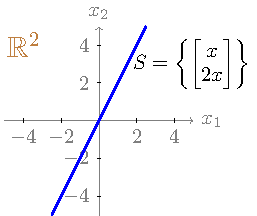
\includegraphics{figure/chapter01/subspace1(a).pdf}
        \caption{A subspace of $\mb{R}^2$.}
        \label{fig:ch01-subspace1}
    \end{subfigure}
    \begin{subfigure}[b]{0.32\textwidth}
        \centering
        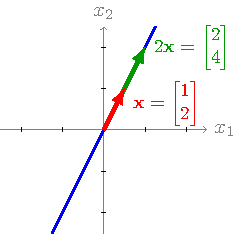
\includegraphics{figure/chapter01/subspace1(b).pdf}
        \caption{Vector scaling.}
        \label{fig:ch01-subspace1-scale}
    \end{subfigure}
    \begin{subfigure}[b]{0.32\textwidth}
        \centering
        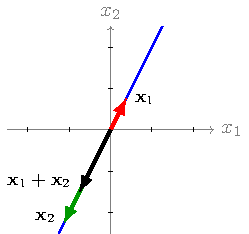
\includegraphics{figure/chapter01/subspace1(c).pdf}
        \caption{Vector addition.}
        \label{fig:ch01-subspace1-addition}
    \end{subfigure}
    \caption{Example of a subspace of $\mb{R}^2$. (a) Shows the set of all points in $\mb{R}^2$ corresponding to the subset $S = \left\{ \bmxc x \\ 2 x\emx\right\} \subset \mb{R}^2$. (b) Shows that the set $S$ is closed under scalar multiplication. Take any vector from the line, and scale it, and it remains on that blue line. (c) Shows that $S$ is closed under vector addition. If we take any two vectors from the blue line and add them, the resulting vector remains in the blue line.}
\end{figure}    
    
\begin{boxedstuff}
\begin{example}
    \textbf{A straight line not through the origin.} Consider the set of all points in $\mb{R}^2$ of the following form:
    \[ S = \lc \mf{x} \, : \, x = \bmxc x \\ m x + c \emx \in \mb{R}^2, \, m, c \in \mb{R} \rc \]
    This is shown in the Figure~\ref{fig:ch01-nosubspace1}.

    How do we verify this is a subspace of $\mb{R}^2$? The definition above shows that any $x$ in $S$ comes from $\mb{R}^2$, which means it is a subset of $\mb{R}^2$. Figure~\ref{fig:ch01-nosubspace1} shows the set $S$ for $m = -\frac{1}{2}$ and $c = 1$.
    \noindent How do we verify if $S$ is a subspace of $\mb{R}^2$? We need to now verify that $S$ satisfies the properties of a vector space.
    \begin{enumerate}
        \item First, let's check if $S$ contains the zero vector. If it does not contain the zero vector, then it cannot be a subspace. The elements from $S$ are of the form $\bmxc x \\ m x + c\emx$, thus if we choose $x = 0$, then we get $\bmx 0 \\ c \emx \in S$. So, $S$ does not contain the zero vector, which implies that $S$ is not a subspace space of $\mb{R}^2$. We need not check the other two conditions, but we will test them just to see which of these two fails.
        \item Scaling the element $\bmxc x \\ m x + c \emx \in S$ by a scalar $d$ we get,
        \[ d \bmxc x \\ m x + c\emx = \bmxc d x \\ d m x + d c \emx = \bmxc d x \\ m \pp{d x} + dc \emx \neq \bmxc y \\ m y + c\emx, \quad \text{where} \,\, y = d x \in \mb{R} \]
        This means that $d \bmxc x \\ m x + c\emx \notin S$. Thus, the set $S$ is not closed under scalar multiplication. Another confirmation that it is not a subspace. This can be seen in Figure~\ref{fig:ch01-nosubspace1-scale}, which shows that when we choose an element from $\mf{x}$ (red arrow) from $S$ (blue line), the scaled version of this vector leaves the set $S$, i.e., the tip of the green arrow does not stay on the blue line.
        \item Let's verify vector addition. Adding two elements $\bmxc x_1 \\ m x_1 + c\emx, \bmxc x_2 \\ m x_2 + c\emx \in S$ we get,
        \[ \bmxc x_1 \\ m x_1 + c\emx + \bmxc x_2 \\ m x_2 + c\emx = \bmxc x_1 + x_2 \\ m x_1 + m x_2 + 2c \emx \neq \bmxc y_1 \\ m y_1 + c\emx, \quad \text{where} \,\, y_1 = x_1 + x_2 \in \mb{R} \]
        This means that $\bmxc x_1 \\ m x_1 + c\emx + \bmxc x_2 \\ m x_2 + c\emx \notin S$. Thus, the set $S$ is not closed under vector addition. We see this geometrically in Figure~\ref{fig:ch01-nosubspace1-addition}, where the sum of two vectors in $S$ does not stay in the set $S$. Even though the tips of the green and red arrows are on the blue line, the tip of the black arrow is not on the blue line.
    \end{enumerate}
    Since the subset $S$ is not closed under both vector addition and scalar multiplication, it is not a subspace of $\mb{R}^2$.
    \label{example:nosubspace-straight-line}
\end{example}
\end{boxedstuff}
\begin{figure}[h]
    \centering
    \begin{subfigure}[b]{0.32\textwidth}
        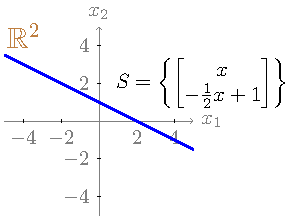
\includegraphics{figure/chapter01/nosubspace1(a).pdf}
        \caption{Not a subspace of $\mb{R}^2$.}
        \label{fig:ch01-nosubspace1}
    \end{subfigure}
    \begin{subfigure}[b]{0.32\textwidth}
        \centering
        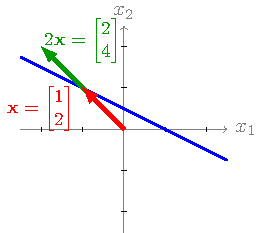
\includegraphics{figure/chapter01/nosubspace1(b).pdf}
        \caption{Vector scaling.}
        \label{fig:ch01-nosubspace1-scale}
    \end{subfigure}
    \begin{subfigure}[b]{0.32\textwidth}
        \centering
        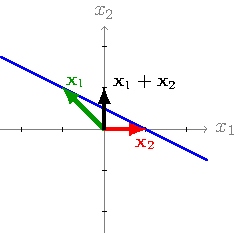
\includegraphics{figure/chapter01/nosubspace1(c).pdf}
        \caption{Vector addition.}
        \label{fig:ch01-nosubspace1-addition}
    \end{subfigure}
    % caption needs to be modified
    \caption{Example of not a subspace of $\mb{R}$. (a) Shows the set of all points in $\mb{R}^2$ corresponding to the subset $S = \left\{ \bmxc x \\ 2 x\emx\right\} \subset \mb{R}^2$. (b) Shows that the set $S$ is closed under scalar multiplication. Take any vector from the line, and scale it, and it remains on that blue line. (c) Shows that $S$ is closed under vector addition. If we take any two vectors from the blue line and add them, the resulting vector remains in the blue line.}
\end{figure}

\begin{boxedstuff}
\begin{example}
    \textbf{A parabola through the origin.} Consider the set of all points in $\mb{R}^2$ of the following form:
    \[ S = \lc \mf{x} \, : \, x = \bmxc x \\ \frac{1}{2}x^2 \emx \in \mb{R}^2, \, m, c \in \mb{R} \rc \]

    This is not a subspace of $\mb{R}^2$. This is geometrically depicted in Figure~\ref{fig:ch01-nosubspace2}, Figure~\ref{fig:ch01-nosubspace2-scale} and Figure~\ref{fig:ch01-nosubspace2-addition}. You are encouraged to verify this algebraically by checking the properties of a vector space.
    \label{example:nosubspace-parabola}
\end{example}
\end{boxedstuff}
\begin{figure}[h]
    \centering
    \begin{subfigure}[b]{0.32\textwidth}
        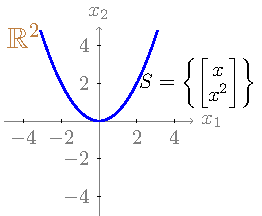
\includegraphics{figure/chapter01/nosubspace2(a).pdf}
        \caption{Not a subspace of $\mb{R}^2$.}
        \label{fig:ch01-nosubspace2}
    \end{subfigure}
    \begin{subfigure}[b]{0.32\textwidth}
        \centering
        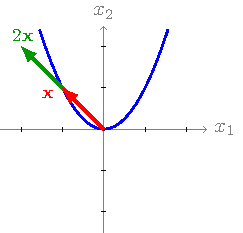
\includegraphics{figure/chapter01/nosubspace2(b).pdf}
        \caption{Vector scaling.}
        \label{fig:ch01-nosubspace2-scale}
    \end{subfigure}
    \begin{subfigure}[b]{0.32\textwidth}
        \centering
        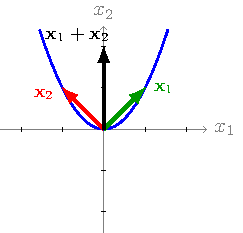
\includegraphics{figure/chapter01/nosubspace2(c).pdf}
        \caption{Vector addition.}
        \label{fig:ch01-nosubspace2-addition}
    \end{subfigure}
    \caption{Example of a subspace of $\mb{R}$. (a) Shows the set of all points in $\mb{R}^2$ corresponding to the subset $S = \left\{ \bmxc x \\ 2 x\emx\right\} \subset \mb{R}^2$. (b) Shows that the set $S$ is closed under scalar multiplication. Take any vecotr from the line, and scale it and it remains on that blue line. (c) Shows that $S$ is closed under vector addition. If we take any two vectors from the blue line and add them, the resulting vector remains in the blue line.}
\end{figure}

\section{Linear combination}
Linear combination is an \textit{algebraic operation} performed on a set of vectors. We can combine the two fundamental operations on vectors into a single operation called the \textit{linear combination} of a set of vectors. Given a set of vectors $\mf{v}_1, \mf{v}_2, \ldots, \mf{v}_m \in \mb{R}^n$ and scalars $c_1, c_2, \ldots, c_n \in \mb{R}$, the linear combination of the vectors is given by:
\begin{equation}
    \mf{v} = c_1 \mf{v}_1 + c_2 \mf{v}_2 + \cdots + c_n \mf{v}_m \in \mb{R}^n
    \label{eq:linear-comb}
\end{equation}
Notice that the linear combinations of single vector $\mf{v}_1$ are simply differently scaled versions of the vector $c_1 \mf{v}_1$. Linear combinations are the bread-and-butter of linear algebra, and we will encounter them again and again. An informal way to think of a linear combination of a set of vectors is the process of mixing the set of vectors together with the corresponding scalar $c_i$, determining the amount of a vector in the mixture. There are other types of combinations of vectors, which we will not discuss further in this book.
\begin{itemize}
    \item \textbf{Affine combination:} $\mf{v} = c_1 \mf{v}_1 + c_2 \mf{v}_2 + \cdots + c_n \mf{v}_m, \quad \sum_{i=1}^{m} c_i = 1$
    \item \textbf{Convex combinations:} $\mf{v} = c_1 \mf{v}_1 + c_2 \mf{v}_2 + \cdots + c_n \mf{v}_m, \quad c_i \geq 0, \,\, \sum_{i=1}^{m} c_i = 1$
    \item \textbf{Conic combinations:} $\mf{v} = c_1 \mf{v}_1 + c_2 \mf{v}_2 + \cdots + c_n \mf{v}_m, \quad c_i \geq 0$
\end{itemize}

\section{Linear independence of a set of vectors}
\secsum{
    \begin{itemize}
        \item Linear independence is a property of a set of vectors.
        \item A set is either linear independent or it's not.
        \item No element of a linearly independent set can be represented as a linear combination of the other elements in the set.
        \item Linearly independent set does not have any redundancy.
    \end{itemize}
}
Linear independence is a \textit{property} of a set of vectors; a set of vectors is either linearly independent or linearly dependent. The concept of linear independence is easy to understand, but the algebraic condition for independence can seem a bit unintuitive. A set of vectors is said to be \text{linearly independent} if no vector in the set can be expressed as a linear combination of the other vectors in the set. This means that there is some unique  information contained in each element of the set, which cannot be obtained from the other elements of the set, i.e., there is no redundancy, so to speak. 

More formally, a set of vectors $V = \lc \mf{v}_i \rc_{i=1}^{m}$ is said to be linearly independent if and only if the only way to produce the zero vector $\mf{0}$ through the linear combination of the set $V$ is by setting all the scalars to zero, i.e.,
\begin{equation}
    c_1 \mf{v}_1 + c_2 \mf{v}_2 + \cdots + c_n \mf{v}_m = \mf{0} \quad \text{if and only if} \quad c_1 = c_2 = \cdots = c_m = 0
    \label{eq:linear-indep}
\end{equation}
To understand this better, let's assume that the set $V$ is linearly dependent, and let's assume that the vector $\mf{v}_m$ can be represented as the linear combination of the vectors $\mf{v}_1, \mf{v}_2, \cdots \mf{v}_{m-1}$. This means that there exist a set of scalar $\alpha_i, \,\, 1 \leq i \leq m-1$, such that
\[ \alpha_1 \mf{v}_1 + \alpha_2 \mf{v}_2 + \cdots + \alpha_{m-1}\mf{v}_{m-1} = \mf{v}_m \]
We can rewrite this as the following,
\[ \begin{split}
    \alpha_1 \mf{v}_1 + \alpha_2 \mf{v}_2 + \cdots + \alpha_{m-1}\mf{v}_{m-1} - \mf{v}_m = \mf{0} \\
    \implies c_m\alpha_1 \mf{v}_1 + c_m\alpha_2 \mf{v}_2 + \cdots + c_m\alpha_{m-1}\mf{v}_{m-1} - c_m\mf{v}_m &= \mf{0}
\end{split} \]
This implies that there exist a set of scalar $c_i = \alpha_i, \,\, 1 \leq i \leq m-1$, and $c_m = -1$ such that $\sum_{i=1}^nc_i \mf{v}_i = \mf{0}$, where not all $c_i$ are zero. So when a set is linearly dependent, then there are scalars $c_i$, not all zero, such that the linear combination of the vectors from $V$ with these scalars produces the zero vector.

Now, let's assume that the set $V$ is linearly independent, that is no vector in the set $V$ can be expressed as a linear combination of other vectors in that set. And let's assume that there are scalars $c_i$, not all zero, such that the linear combination of the vectors from $V$ with these scalars produces the zero vector, i.e.,
\[ \begin{split}
    c_1 \mf{v}_1 + c_2 \mf{v}_2 + \cdots + c_m \mf{v}_m &= \mf{0} \\
    \implies \frac{c_1}{c_m} \mf{v}_1 + \frac{c_2}{c_m} \mf{v}_2 + \cdots + \frac{c_{m-1}}{c_m}\mf{v}_{m-1} &= \mf{v}_m, \,\, c_m \neq 0
\end{split} \]
But this a contradiction because we have just expressed $\mf{v}_m$ as a linear combination of the vectors $\mf{v}_1, \mf{v}_2, \cdots \mf{v}_{m-1}$.

\begin{boxedstuff}
    \begin{example}
        Consider the set of vectors $\lc \mf{v}_1, \mf{v}_2 \rc$, such that $\mf{v}_1 = \bmx 1 \\ 0 \emx, \mf{v}_2 = \bmx 0 \\ 1 \emx$ in $\mb{R}^2$. This set is linearly independent. Let's verify this algebraically. Let's assume that there exist scalars $c_1, c_2$ such that $c_1 \mf{v}_1 + c_2 \mf{v}_2 = \mf{0}$. This implies that, $c_1 \bmx 1 \\ 0 \emx + c_2 \bmx 0 \\ 1 \emx = \bmx c_1 \\ c_2 \emx = \bmx 0 \\ 0 \emx \implies c_1 = c_2 = 0$. Thus the set $\lc \mf{v}_1, \mf{v}_2 \rc$ is linearly independent. 
    \end{example}

    \begin{example}
        Consider the set of vectors $\lc \mf{v}_1, \mf{v}_2 \rc$, such that $\mf{v}_1 = \bmx 1 \\ 0 \emx, \mf{v}_2 = \bmx 0 \\ 1 \emx, , \mf{v}_3 = \bmx 23 \\ -5 \emx$ in $\mb{R}^2$. This set is not linearly independent, i.e., its linear dependent. Let's assume that there exist scalars $c_1, c_2, c_3$ such that $c_1 \mf{v}_1 + c_2 \mf{v}_2 + c_3 \mf{v}_3 = \mf{0}$. This implies that, $c_1 \bmx 1 \\ 0 \emx + c_2 \bmx 0 \\ 1 \emx + c_3 \bmx 23 \\ -5 \emx = \bmx c_1 + 23c_3\\ c_2  - 5 c_3 \emx = \bmx 0 \\ 0 \emx \implies c_1 = -23c_3$ and $c_2 = 5c_3$. If we choose $c_3$ to be a non-zero value, we have a set of non-zero scalars such that a linear combination of the set $\lc \mf{v}_1, \mf{v}_2, \mf{v}_3 \rc$ produces the zero vector. Thus, this set is linearly dependent.
    \end{example}

    \begin{example}
        Consider the set of vectors $\lc \mf{v}_1 \rc$, $\mf{v}_1 = \bmx -1 \\ 1 \\ 1 \emx$ in $\mb{R}^3$. This set is linearly independent. Let's assume that there exist scalars $c_1$ such that $c_1 \mf{v}_1 = \mf{0}$. This implies that, $\bmx -c_1 \\ c_1 \\ c_1 \emx = \bmx 0 \\ 0 \\ 0 \emx \implies c_1 = 0$. Thus, the set $\lc \mf{v}_1 \rc$ is linearly independent.
    \end{example}

    \begin{example}
        Consider the set $\lc \mf{0} \rc$ in $\mb{R}^3$. This set is linearly dependent. Here, $c_1 \mf{0} = \bmx 0 c_1 \\ 0 c_1 \\ 0 c_1 \emx = \mf{0}$. Any non-zero $c_1$ will produce the zero vector. Thus, the set $\lc \mf{v}_1 \rc$ is linearly dependent. In fact, any set that contains the zero vector is linearly dependent. \textcolor{blue}{(Why? Can you show this algebraically?)}
    \end{example}
\end{boxedstuff}

\section{Span of a set of vectors}\label{sec:ch01-span}
\secsum{
    \begin{itemize}
        \item The span of a set of vectors $V$ is another set.
        \item It is generated through the linear combination of the elements of $V$.
        \item The span of a set of vectors $V$ is a subspace of the original vector space the elements of $V$ are from.
    \end{itemize}
}
So, linear combinations of a set of vectors $V = \lc \mf{v}_i \rc_{i=1}^{m}$ ($\mf{v}_i \in \mb{R}^n$) is a way of generating new vectors not in that set. All we need to do is choose a random set of real numbers $\lc c_i \rc_{i=1}^{m}$, and ``mix'' the vectors $\mf{v}_i$ from the set using these as weights. Clearly, there are an infinite number of vectors we could generate through this process, and we can put them all together in a set. And this set has a name -- the \textit{span} of the set $V$. The span of a set of vectors $V = \lc \mf{v}_i \rc_{i=1}^{m}$ is denoted by $\text{span}\lp V \rp$ and is defined as:
\begin{equation}
    \text{span}\lp V \rp = \lc c_1 \mf{v}_1 + c_2 \mf{v}_2 + \cdots + c_n \mf{v}_m \, : \, c_i \in \mb{R} \rc \subseteq \mb{R}^n
    \label{eq:span-vec}
\end{equation}
It's clear that this will be a subset of $\mb{R}^n$, but it turns out that it is also a subspace of $\mb{R}^n$. Why? Can you verify this fact algebraically? (\textit{Hint}: Just follow the steps in Examples~\ref{example:subspace-straight-line}-\ref{example:nosubspace-parabola}).

Geometrically, this means that the $\text{span}\pp{V}$ will be a flat surface in $\mb{R}^n$. This means that the linear combination operation generates vectors that lie on a flat surface spanned by the vectors employed in the linear combination.

\begin{figure}[h]
    \centering
    \begin{subfigure}[b]{0.32\textwidth}
        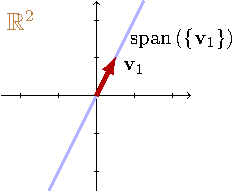
\includegraphics{figure/chapter01/span(a).pdf}
        \caption{Not a subspace of $\mb{R}^2$.}
        \label{fig:ch01-span1}
    \end{subfigure}
    \begin{subfigure}[b]{0.32\textwidth}
        \centering
        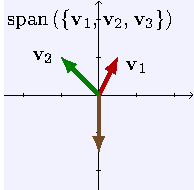
\includegraphics{figure/chapter01/span(b).pdf}
        \caption{Vector scaling.}
        \label{fig:ch01-span2}
    \end{subfigure}
    \begin{subfigure}[b]{0.32\textwidth}
        \centering
        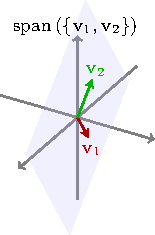
\includegraphics{figure/chapter01/span(c).pdf}
        \caption{Vector addition.}
        \label{fig:ch01-span3}
    \end{subfigure}
    \caption{Span of a set of vectors in $\mb{R}^2$ and $\mb{R}^3$.}
\end{figure}

\section{How big is a vector?}
The size of a vector is an extension of the idea of the magnitude of a real number. The magnitude of a real number $a \in \mb{R}$ tells us how big the number is irrespective of its sign:
\begin{equation}
    \vert a \vert = \begin{cases} a, & a \geq 0 \\ -a, & a < 0 \end{cases}
    \label{eq:magnitude-real}
\end{equation}

The ``magnitude'' or size of an element of a vector space (such as $\mb{R}^n$) is called the \textit{norm} of the vector. The norm is a generalization of the magnitude of a real number to a vector. The norm of a vector is a function that maps a vector to a non-negative real number and satisfies the following properties:
\begin{itemize}
    \item \textbf{Non-negativity:} For any vector $\mf{x} \in \mb{R}^n$, $\norm{\mf{x}} \geq 0$.
    \item \textbf{Definiteness:} The norm of a vector is zero if and only if the vector is the zero vector, i.e., $\norm{\mf{x}} = 0$ if and only if $\mf{x} = \mf{0}$.
    \item \textbf{Homogeneity:} Scaling a vector by a scalar $c$, scales the norm of the vector by $\vert c \vert$. For any vector $\mf{x} \in \mb{R}^n$ and any scalar $c \in \mb{R}$, $\norm{c\mf{x}} = \vert c \vert \norm{\mf{x}}$.
    \item \textbf{Triangle inequality:} For any vectors $\mf{x}, \mf{y} \in \mb{R}^n$, $\norm{\mf{x} + \mf{y}} \leq \norm{\mf{x}} + \norm{\mf{y}}$.
\end{itemize}
According to this definition, the magnitude of real numbers (Eq.~\ref{eq:magnitude-real}) is a norm of the vector space $\mb{R}$. The most common norm of a vector is the \textit{Euclidean norm} or the \textit{2-norm} of a vector. The Euclidean norm of a vector $\mf{x} = \bmxc x_1 \\ x_2 \\ \vdots \\ x_n \emx$ is defined as:
\begin{equation}
    \norm{\mf{x}}_2 = \sqrt{x_1^2 + x_2^2 + \cdots + x_n^2}
    \label{eq:euclidean-norm}
\end{equation}
We are well-versed with this as the length of a vector in $\mb{R}^2$ and $\mb{R}^3$. The properties of non-negativity, definiteness, and homogeneity are easy to verify. The triangle inequality is a bit more involved.

The subscript $2$ in Eq.~\ref{eq:euclidean-norm} is used to indicate that it is the 2-norm, which is a special case of a general class of norms in $\mb{R}^n$ -- the \textit{p-norm}. The \textit{p-norm} is defined as the following:
\begin{equation}
    \norm{\mf{x}}_p = \lp \sum_{i=1}^{n} \vert x_i \vert^p \rp^{1/p}, \,\, p \in \mb{Z}, \,\, p \geq 1
    \label{eq:p-norm}
\end{equation}
Apart from the \textit{2-norm}, the \textit{1-norm} and the \textit{$\infty$-norm} are also commonly used norms, which are defined as the following:
\begin{equation}
    \norm{\mf{x}}_1 = \sum_{i=1}^{n} \vert x_i \vert, \quad \quad \quad \norm{\mf{x}}_{\infty} = \max_{i} \vert x_i \vert
    \label{eq:1-infinity-norm}
\end{equation}
The \textit{1-norm} is the sum of the absolute value of the elements of the vector, and the \textit{$\infty$-norm} is the maximum of the absolute value of the elements of the vector. The \textit{1-norm} is also called the \textit{Manhattan norm} or the \textit{Taxicab norm} because it measures the distance between two points in a city if you can only travel along the grid of streets.

\begin{boxedstuff}
    \begin{example}
        Let's calculate the 1-norm, 2-norm, and $\infty$-norm of the some vectors: %$\mf{x}_1 = \bmxc 1 \\ 2 \\ 3 \emx$, $\mf{x}_2 = \bmxc 0 \\ 3 \\ 4 \emx$, $\mf{e}_1 = \bmxc 1 \\ 0 \\ 0 \emx$, $\mf{e}_2 = \bmxc 0 \\ 1 \\ 0 \emx$, .

        \begin{enumerate}
            \item $\mf{x}_1 = \bmxc 1 \\ -1 \\ 3 \emx \longrightarrow \lV \mf{x}_1 \rV_1 = 5, \quad \lV \mf{x}_1 \rV_2 = \sqrt{1 + 1 + 9} = \sqrt{11}, \quad \lV \mf{x}_1 \rV_{\infty} = 3$.
            \item $\mf{e}_2 = \bmxc 0 \\ 1 \\ 0 \emx \longrightarrow \lV \mf{x}_1 \rV_1 = 1, \quad \lV \mf{x}_1 \rV_2 = 1, \quad \lV \mf{x}_1 \rV_{\infty} = 1$. All the $p$-norms of the unit vectors are $1$. No wonder we call them ``unit'' vectors.
            \item $\lV \mf{0} \rV_1 = \lV \mf{0} \rV_2 = \lV \mf{0} \rV_{\infty} = 0$. All $p$-norms will produce 0, otherwise it is not a norm (remember the definiteness property?)
        \end{enumerate}
    \end{example}
\end{boxedstuff}

\begin{boxedstuff}
    \begin{problem}
        Why does the $\infty$-norm measure have this weird-looking definition compared to the other $p$-norms?
        \begin{solution}
            Consider the vector $\mf{x} \in \mb{R}^n$, and $x_{max} = \max_{0 \leq i \leq n} \vert x_i \vert$; let's also assume that the $j^{th}$ element of $\mf{x}$ has the maximum absolute value, i.e. $x_{max} = \vert x_j \vert$. The $p$-norm is defined as the following:
            \[ \begin{split} 
                \norm{\mf{x}}_p &= \lp \sum_{i=1}^{n} \vert x_i \vert^p \rp^{1/p} = x_{max} \lp 1 + \sum_{\substack{1 \leq i \leq n \\ i \neq j}} \lv \frac{x_i}{x_j} \rv^p \rp^{1/p} = x_{max}\lp N \rp^{1/p}\\
            \end{split}
            \]
            where, $N$ is a real number between $1$ and $n$, because $\vert \frac{x_i}{x_j} \vert \leq 1$ (why?). Now, if we increase the value of $p$ to infinity, then the term $\lim_{p \to infty} \lp N \rp^{1/p}= 1$. Thus, we have $\lV \mf{x} \rV_{\infty} = \lim_{p \to \infty} \lV \mf{x} \rV_p = x_{max} = \max_{i} \lv x_i \rv$.
        \end{solution}
    \end{problem}
\end{boxedstuff}

\subsection{Geometry of the p-norms}
In the case of real numbers, the set of all numbers with a magnitude of $1$ is the set $\lc -1, 1 \rc$. We can plot these points in the real line as below.

% Figure showing the locus of all points with magnitude 1
% on the real line.
\begin{figure}[h]
    \centering
    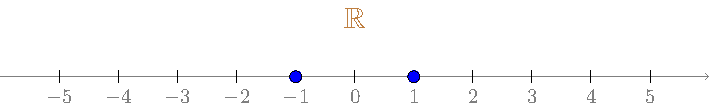
\includegraphics{figure/chapter01/mag-locus.pdf}
    \caption{The set of all real numbers with magnitude $1$. This set contains two numbers $\lc -1, 1 \rc$.}
    \label{fig:ch01-real-line-1-norm}
\end{figure}

In $\mb{R}^2$, the set of all vectors from $\mb{R}^2$ with a \textit{2-norm} of $1$ is the unit circle. The following figure shows the set of all points in $\mb{R}^2$ with units 1, 2, $p$, and $\infty$ norm.
\begin{figure}[h]
    \centering
    \begin{subfigure}[b]{0.24\textwidth}
        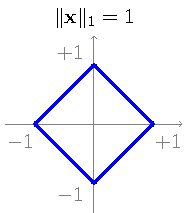
\includegraphics{figure/chapter01/norm1.pdf}
        \caption{1-norm}
        \label{fig:ch01-norm1}
    \end{subfigure}
    \begin{subfigure}[b]{0.24\textwidth}
        \centering
        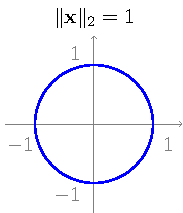
\includegraphics{figure/chapter01/norm2.pdf}
        \caption{2-norm}
        \label{fig:ch01-norm2}
    \end{subfigure}
    \begin{subfigure}[b]{0.24\textwidth}
        \centering
        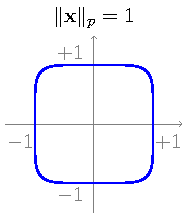
\includegraphics{figure/chapter01/normp.pdf}
        \caption{$p$-norm}
        \label{fig:ch01-normp}
    \end{subfigure}
    \begin{subfigure}[b]{0.24\textwidth}
        \centering
        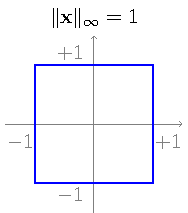
\includegraphics{figure/chapter01/norminf.pdf}
        \caption{$\infty$-norm}
        \label{fig:ch01-norminf}
    \end{subfigure}
    \caption{Locus of all points with unit 1, 2, $p$, and $\infty$ norms in $\mb{R}^2$.}
\end{figure}

\begin{boxedstuff}
    \begin{problem}
        Can you explain why the different norms have these shapes? 
    \end{problem}
    \begin{problem}
        Can you write a Python program to generate the above plots for different values of $p = 1, 2, 3, 10$ and $\infty$?
    \end{problem}
    \begin{problem}
        Can describe what these 1, 2, $p$ and $\infty$ norms will look like in $\mb{R}^3$?
    \end{problem}
\end{boxedstuff}

\section{How similar are two vectors?}\label{sec:ch01-similar-vecs}
The idea of how similar two or more vectors are is an important topic  in data analysis, in particular in classification problems in machine learning. Vectors that are ``similar'' somehow belong to the same ``category'' or ``class'', while vectors that are ``dissimilar'' belong to different categories or classes. There are various ways to measure the similarity between two vectors. We will look at two methods in this section where similarity is measured by computing the distance between two vectors or by computing the angle between two vectors.

\subsection{Distance between two vectors}
The logic here is that similar vectors correspond to points that are close together, while dissimilar vectors are farther away. We can make use of the norm to compute the distance between two vectors $\mf{x}, \mf{y} \in \mb{R}^n$. Since the difference between these two vectors $\mf{x} - \mf{y}$ is also another vector, we can compute the distance between vectors $\mf{x}$ and $\mf{y}$ as the norm of the vector $\mf{x} - \mf{y}$ (Figure~\ref{fig:ch01-dist1}).
\[ \text{Distance between } \mf{x} \text{ and } \mf{y} = d\pp{\mf{x}, \mf{y}} = \lV \mf{x} - \mf{y} \rV_p \]
We could use any of the $p$-norms to compute this or come up with a new norm depending on the application we are dealing with. Take a look at the clusters of points shown in Figure~\ref{fig:ch01-dist-clusters}, we would agree that the different colored points each form a cluster, since the points of the same color are closer to each other than points from another color. 

\begin{boxedstuff}
    \begin{example}
        \textbf{Test scores in ALADA}. The ALADA course has three segments: linear algebra, optimization, and probability/statistics. Let's assume that the final exam contains three sections with a maximum of 25 marks students. The scores from these three segments are stored in a $3$-vector of the form $\mf{x} = \bmxc x_1 \\ x_2 \\ x_3\emx \in \mb{R}^3$, where $x_1, x_2, x_3$ are the marks obtained for linear algebra, optimization, and probability/statistics section, respectively. Consider the scores from the 6 students who took the course:
        \[ \mf{x}_1 = \bmxc 2 \\ 5 \\ 1 \emx, \quad \mf{x}_2 = \bmxc 3 \\ 3 \\ 4 \emx, \quad \mf{x}_3 = \bmxc 8 \\ 20 \\ 22 \emx, \quad \mf{x}_4 = \bmxc 9 \\ 20 \\ 21 \emx, \quad \mf{x}_5 = \bmxc 24 \\ 24 \\ 23 \emx, \quad \mf{x}_6 = \bmxc 24 \\ 23 \\ 22 \emx
        \]
        The distance between the scores of these students tells us something about the ability of the students in the course. Let $d_{ij} = \lV \mf{x}_i - \mf{x}_j \rV_2$ be the Euclidean distance between the scores of student $i$ and $j$; notice that $d_{ij} = d_{ji}$. The distance between the different scores is given by the following table. \\
        \begin{small}
            \begin{center}
            \begin{tabular}{lc|cccccc|}
                \cline{3-8}
                & \multicolumn{1}{l|}{} & \multicolumn{6}{c|}{$\mathbf{x}_i$} \\ \cline{3-8} 
                &  & \multicolumn{1}{c|}{1} & \multicolumn{1}{c|}{2} & \multicolumn{1}{c|}{3} & \multicolumn{1}{c|}{4} & \multicolumn{1}{c|}{5} & 6 \\ \hline
                \multicolumn{1}{|l|}{\multirow{6}{*}{$\mathbf{x}_j$}} & 1 & \multicolumn{1}{c|}{0.0} & \multicolumn{1}{c|}{3.7} & \multicolumn{1}{c|}{26.5} & \multicolumn{1}{c|}{26.0} & \multicolumn{1}{c|}{36.5} & 35.3 \\ \cline{2-8} 
                \multicolumn{1}{|l|}{} & 2 & \multicolumn{1}{c|}{\textcolor{gray}{$\theta_{12}$}} & \multicolumn{1}{c|}{0.0} & \multicolumn{1}{c|}{25.3} & \multicolumn{1}{c|}{24.8} & \multicolumn{1}{c|}{35.3} & 34.1 \\ \cline{2-8} 
                \multicolumn{1}{|l|}{} & 3 & \multicolumn{1}{c|}{\textcolor{gray}{$\theta_{13}$}} & \multicolumn{1}{c|}{\textcolor{gray}{$\theta_{23}$}} & \multicolumn{1}{c|}{0.0} & \multicolumn{1}{c|}{1.4} & \multicolumn{1}{c|}{16.5} & 16.3 \\ \cline{2-8} 
                \multicolumn{1}{|l|}{} & 4 & \multicolumn{1}{c|}{\textcolor{gray}{$\theta_{14}$}} & \multicolumn{1}{c|}{\textcolor{gray}{$\theta_{24}$}} & \multicolumn{1}{c|}{\textcolor{gray}{$\theta_{34}$}} & \multicolumn{1}{c|}{0.0} & \multicolumn{1}{c|}{15.7} & 15.3 \\ \cline{2-8} 
                \multicolumn{1}{|l|}{} & 5 & \multicolumn{1}{c|}{\textcolor{gray}{$\theta_{15}$}} & \multicolumn{1}{c|}{\textcolor{gray}{$\theta_{25}$}} & \multicolumn{1}{c|}{\textcolor{gray}{$\theta_{35}$}} & \multicolumn{1}{c|}{\textcolor{gray}{$\theta_{45}$}} & \multicolumn{1}{c|}{0.0} & 1.4 \\ \cline{2-8} 
                \multicolumn{1}{|l|}{} & 6 & \multicolumn{1}{c|}{\textcolor{gray}{$\theta_{16}$}} & \multicolumn{1}{c|}{\textcolor{gray}{$\theta_{26}$}} & \multicolumn{1}{c|}{\textcolor{gray}{$\theta_{36}$}} & \multicolumn{1}{c|}{\textcolor{gray}{$\theta_{46}$}} & \multicolumn{1}{c|}{\textcolor{gray}{$\theta_{56}$}} & 0.0 \\ \hline
                \end{tabular}
            \end{center}
        \end{small}
        
        \noindent The following observations can be made from the table:
        \begin{itemize}
            \item Students 1 and 2 have similar scores compared to the other students.
            \item Students 3 and 4 have very similar scores compared to the other students.
            \item Students 5 and 6 have very similar scores compared to the other students.
            \item Students 1 and 2 are closer to 3 and 4 than to 5 and 6.
        \end{itemize}

        \noindent Notice that you could have also used the other norms to create a table similar to the above one. It's left as an exercise for you to generate a similar table using the $1$-norm and the $\infty$-norm to define the distance between the scores of the students.

        \textbf{Using norms instead of norms of differences}. Another way to understand the score vectors is to directly compute the norms of $\mf{x}_i$ and see what information they convey about the students' performance in the ALADA final exam.
        \begin{small}
            \begin{center}
                    \begin{tabular}{|c|c|c|c|c|c|}
                    \hline
                    $\lV \mf{x}_1 \rV_2$ & $\lV \mf{x}_2 \rV_2$ & $\lV \mf{x}_3 \rV_2$ & $\lV \mf{x}_4 \rV_2$ & $\lV \mf{x}_5 \rV_2$ & $\lV \mf{x}_6 \rV_2$ \\ \hline
                    5.5 & 5.8 & 30.8 & 30.4 & 41.0 & 39.9 \\ \hline
                    \end{tabular}
            \end{center}
        \end{small}
        The size of the score vectors tells us that students 1 and 2 performed worst among the six students, while students 5 and 6 performed the best; the performance of students 3 and 4 was somewhere in the middle. \textcolor{blue}{Would we have reached similar conclusions if we had used the $1$-norm or the $\infty$-norm to compute the norms of the score vectors?}
        \label{example:alada-scores}
    \end{example}
\end{boxedstuff}

\begin{figure}[h]
    \centering
    \begin{subfigure}[b]{0.35\textwidth}
        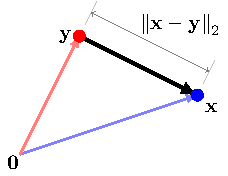
\includegraphics[width=0.95\linewidth]{figure/chapter01/dist-demo.pdf}
        \caption{Distance between two vectors $\mf{x}$ and $\mf{y}$ in $\mb{R}^2$. This figure depicts the 2-norm, but any $p$-norm or valid norm function could be used to quantify the distance between two vectors or points.}
        \label{fig:ch01-dist1}
    \end{subfigure}
    \hspace{0.05\textwidth}
    \begin{subfigure}[b]{0.4\textwidth}
        \centering
        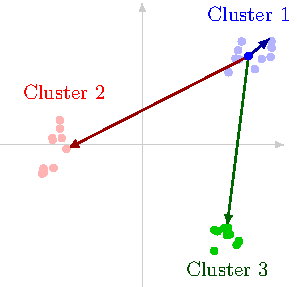
\includegraphics[width=0.85\linewidth]{figure/chapter01/cluster-dist.pdf}
        \caption{Distance between two vectors $\mf{x}$ and $\mf{y}$ in $\mb{R}^2$. This figure depicts the 2-norm, but any $p$-norm or valid norm function could be used to quantify the distance between two vectors or points.  could be used to quantify the distance between}
        \label{fig:ch01-dist-clusters}
    \end{subfigure}
    \caption{}
\end{figure}

\subsection{Angle between two vectors}
This approach is based on the idea that the direction of the vector representing a point contains information about the point. Thus, vectors that point in a similar direction could be considered similar. But how do we measure the angle between two vectors in $\mb{R}^n$? This is where the concept of the \textit{standard inner product} (or the dot product from vectors from high school math and physics). The standard inner product of two vectors $\mf{x}, \mf{y} \in \mb{R}^n$ is defined as:
\[ \mf{x}^\top\mf{y} = \sum_{i=1}^{n} x_i y_i \]
The superscript `$\top$' represents the transpose operation. We will not worry about what it means until the next chapter. The standard inner product takes in two vectors $\mf{x}, \mf{y} \in \mb{R}^n$ and returns a scalar value $\mb{R}$; it can be both positive and negative. We compute it by simply taking the two vectors $\mf{x} = \bmxc x_1 \\ \vdots \\ x_n \emx$ and $\mf{y} = \bmxc y_1 \\ \vdots \\ y_n \emx$, and multiply the two of them element-wise $x_i y_i, \, 1 \leq i \leq n$ and add the $n$ products together $\sum_{i=1}^n x_i y_i$ to obtain the inner product.

\begin{figure}[h]
    \centering
    \begin{subfigure}[b]{0.45\textwidth}
        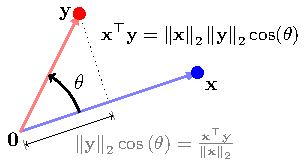
\includegraphics[width=0.95\linewidth]{figure/chapter01/angle-demo.pdf}
        \caption{Angle between two vectors $\mf{x}$ and $\mf{y}$ in $\mb{R}^2$. The standard inner product provides a measure of the cosine of the angle between the two vectors.}
        \label{fig:ch01-angle1}
    \end{subfigure}
    \hspace{0.05\textwidth}
    \begin{subfigure}[b]{0.4\textwidth}
        \centering
        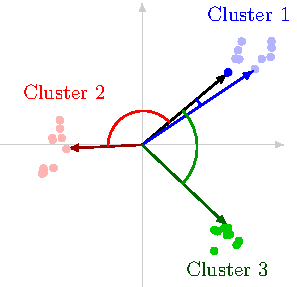
\includegraphics[width=0.85\linewidth]{figure/chapter01/cluster-angle.pdf}
        \caption{The relative angle between the points of the same colors is smaller than that of points of different colors.}
        \label{fig:ch01-angle-clusters}
    \end{subfigure}
    \caption{}
\end{figure}

The standard inner product of two vectors $\mf{x}$ and $\mf{y}$ is related to the cosine of the angle $\theta$ between the two vectors and the 2-norm of the two vectors.
\[ \mf{x}^\top\mf{y} = \sum_{i=1}^n x_i y_i = \lV \mf{x} \rV_2 \cdot \lV \mf{y} \rV_2 \cdot \cos\pp{\theta} \]
The angle $\theta$ between the two vectors $\mf{x}$ and $\mf{y}$ can be computed as:
\[ \theta = \cos^{-1}\pp{\frac{\mf{x}^\top \mf{y}}{\lV \mf{x} \rV_2 \lV \mf{y} \rV_2}}, \,\, \lV \mf{x} \rV_2 \neq 0, \lV \mf{y} \rV_2 \neq 0 \]
If the 2-norms of the $\mf{x}$ and $\mf{y}$, then $\mf{x}^\top\mf{y}$ is simply the cosine of the angle between the vectors.

\begin{boxedstuff}
    \begin{example}
        Let's look at the data from Example~\ref{example:alada-scores}, but this time using the angle between the vectors to understand the performance of the students in the ALADA final exam. The angle between the scores (in degrees) of the students is given in the following table. Let $\theta_{ij} = \cos^{-1}\pp{\frac{\mf{x}_i^\top\mf{x}_j}{\lV \mf{x}_i \rV_2 \lV \mf{x}_j \rV_2}}$ be the angle between the scores of student $i$ and $j$; notice that $\theta_{ij} = \theta_{ji}$.
        \begin{small}
            \begin{center}
            \begin{tabular}{lc|cccccc|}
                \cline{3-8}
                & \multicolumn{1}{l|}{} & \multicolumn{6}{c|}{$\mathbf{x}_i$} \\ \cline{3-8} 
                &  & \multicolumn{1}{c|}{1} & \multicolumn{1}{c|}{2} & \multicolumn{1}{c|}{3} & \multicolumn{1}{c|}{4} & \multicolumn{1}{c|}{5} & 6 \\ \hline
                \multicolumn{1}{|l|}{\multirow{6}{*}{$\mathbf{x}_j$}} & 1 & \multicolumn{1}{c|}{0.0} & \multicolumn{1}{c|}{38.5} & \multicolumn{1}{c|}{35.1} & \multicolumn{1}{c|}{33.3} & \multicolumn{1}{c|}{31.7} & 32.1 \\ \cline{2-8} 
                \multicolumn{1}{|l|}{} & 2 & \multicolumn{1}{c|}{\textcolor{gray}{$\theta_{12}$}} & \multicolumn{1}{c|}{0.0} & \multicolumn{1}{c|}{16.7} & \multicolumn{1}{c|}{15.0} & \multicolumn{1}{c|}{9.2} & 9.9 \\ \cline{2-8} 
                \multicolumn{1}{|l|}{} & 3 & \multicolumn{1}{c|}{\textcolor{gray}{$\theta_{13}$}} & \multicolumn{1}{c|}{\textcolor{gray}{$\theta_{23}$}} & \multicolumn{1}{c|}{0.0} & \multicolumn{1}{c|}{2.5} & \multicolumn{1}{c|}{21.1} & 22.2 \\ \cline{2-8} 
                \multicolumn{1}{|l|}{} & 4 & \multicolumn{1}{c|}{\textcolor{gray}{$\theta_{14}$}} & \multicolumn{1}{c|}{\textcolor{gray}{$\theta_{24}$}} & \multicolumn{1}{c|}{\textcolor{gray}{$\theta_{34}$}} & \multicolumn{1}{c|}{0.0} & \multicolumn{1}{c|}{18.7} & 19.9 \\ \cline{2-8} 
                \multicolumn{1}{|l|}{} & 5 & \multicolumn{1}{c|}{\textcolor{gray}{$\theta_{15}$}} & \multicolumn{1}{c|}{\textcolor{gray}{$\theta_{25}$}} & \multicolumn{1}{c|}{\textcolor{gray}{$\theta_{35}$}} & \multicolumn{1}{c|}{\textcolor{gray}{$\theta_{45}$}} & \multicolumn{1}{c|}{0.0} & 1.2 \\ \cline{2-8} 
                \multicolumn{1}{|l|}{} & 6 & \multicolumn{1}{c|}{\textcolor{gray}{$\theta_{16}$}} & \multicolumn{1}{c|}{\textcolor{gray}{$\theta_{26}$}} & \multicolumn{1}{c|}{\textcolor{gray}{$\theta_{36}$}} & \multicolumn{1}{c|}{\textcolor{gray}{$\theta_{46}$}} & \multicolumn{1}{c|}{\textcolor{gray}{$\theta_{56}$}} & 0.0 \\ \hline
                \end{tabular}
            \end{center}
        \end{small}
    \end{example}
    It looks like the angles do not do a good job of capturing the similarity between the scores of the students like the distance between the scores, in particular $\theta_{12}$ is quite large, while $\theta_{34}$ and $\theta_{56}$ are quite small. \textcolor{blue}{Why do you think this is so?}
\end{boxedstuff}

\section{Standard and other inner products}
$\mf{x}^\top\mf{y}$ is the standard inner product, which of course means there are non-standard inner products. But before we look at generalizing the concept of an inner product, let's look at some properties of the standard inner product.
\begin{itemize}
    \item \textbf{Connection to the 2-norm}. The standard inner product of a vector $\mf{x}$ with itself is the square of the 2-norm of the vector, i.e., $\mf{x}^\top\mf{x} = \lV \mf{x} \rV_2^2 = \sum_{i=1}^n x_i^2$.
    \item \textbf{Cauchy-Bunyakovski-Schwartz Inequality}:
    \begin{equation}
        \mf{x}^\top\mf{y} \leq \lV \mf{x} \rV_2 \lV \mf{y} \rV_2
        \label{eq:cauchy-schwartz}
    \end{equation}
\end{itemize}

The concept of an inner product is a general one. An inner product $\langle \cdot, \cdot \rangle$ is a function that maps two vectors from $\mb{R}^n$ to a scalar value, and satisfies the following properties:
\begin{itemize}
    \item \textbf{Positive definiteness:} $\langle \mf{x}, \mf{x} \rangle \geq 0$, and $\langle \mf{x}, \mf{x} \rangle = 0$ if and only if $\mf{x} = \mf{0}$.
    \item \textbf{Symmetry:} For any vectors $\mf{x}, \mf{y}$, $\langle \mf{x}, \mf{y} \rangle = \langle \mf{y}, \mf{x} \rangle$.
    \item \textbf{Linearity:} For any vectors $\mf{x}, \mf{y}$, $\mf{z}$, and any scalars $\alpha, \beta \in \mb{R}$, $\langle \alpha\mf{x} + \beta \mf{y}, \mf{z} \rangle = \alpha \langle \mf{x}, \mf{y}\rangle + \beta \langle \mf{y}, \mf{z}\rangle$.
\end{itemize}
We will come across other inner products in due course, but we will stick to the standard inner product for most problems in $\mb{R}^n$ in this course. A class of inner products in $\mb{R}^n$ is of the form $\langle \mf{x}, \mf{y}\rangle = \mf{x}^\top\mf{A}\mf{y}$, where $\mf{A}$ is a $n \times n$ \textit{positive definite} matrix. The standard inner product is a special case of this class of inner products where $\mf{A} = \mf{I}$, the identity matrix. That may sound like too much jargon for now, but we will come to these concepts in the upcoming chapters.

\begin{boxedstuff}
\begin{problem}
    Consider the vector space $\mb{R}^n$. Is the following a valid inner product of $\mb{R}^n$?
    \[ \langle \mf{x}, \mf{y}\rangle = \sum_{i=1}^n w_1 x_i y_i, \,\, w_i \in \mb{R}, \,\, w_i > 0 \]
    \begin{solution}
        To find out if this is a valid inner product, we need to verify by if it satisfies the properties of an inner product. 
        \begin{itemize}
            \item \textbf{Positive definiteness}: The first property is positive definiteness, which is satisfied because $w_i > 0$.
            \[ \langle \mf{x}, \mf{x} \rangle = \sum_{i=1}^n w_i x_i^2 \geq 0, \,\, \text{since, } w_i > 0 \text{ and } x_i^2 \geq 0 \]
            Notice that if any of the $w_i$ is zero or negative, then $\langle \mf{x}, \mf{y} \rangle$ will not be a valid inner product (why?).
            \item \textbf{Symmetry}: From the commutativity and associativity of multiplication of real numbers, we have $\langle \mf{x}, \mf{y} \rangle = \langle \mf{y}, \mf{x} \rangle$. 
        
            \item\textbf{Linearity}: This is also satisfied. You should verify this yourself.
        \end{itemize}
        The given function is a valid inner product of $\mb{R}^n$.
    \end{solution}
\end{problem}
\begin{problem}
    Consider the vector space $\mb{R}^n$. Is the following a valid inner product of $\mb{R}^n$?
    \[ \langle \mf{x}, \mf{y}\rangle = \sum_{i=1}^n w_i x_i y_i, \,\, w_i = \begin{cases} +1, & i \text{ is odd} \\  -1, & i \text{ is even}\end{cases} \]
    \begin{solution}
        To find out if this is a valid inner product, we need to verify if it satisfies the properties of an inner product. 
        \begin{itemize}
            \item \textbf{Positive definiteness}: This is not satisfied. Can you provide an example where positive definiteness fails?
        \end{itemize}
        The given function is a \textit{not} valid inner product of $\mb{R}^n$.
    \end{solution}
\end{problem}
\end{boxedstuff}

\section{Orthogonality of vectors}

% Floating figure to the right of the text
\begin{wrapfigure}{r}{0.4\textwidth}
    \centering
    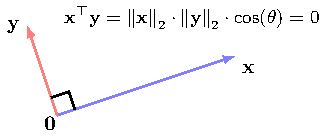
\includegraphics[width=0.35\textwidth]{figure/chapter01/ortho-demo.pdf}
    \caption{Orthogonal vectors in $\mb{R}^2$.}
    \label{fig:ch01-orthog-vectors}
\end{wrapfigure}
The concept of orthogonality is a generalization of the concept of perpendicularity in $\mb{R}^2$ and $\mb{R}^3$. Two vectors $\mf{x}, \mf{y} \in \mb{R}^n$ are said to be orthogonal if their standard inner product is zero, i.e., $\mf{x}^\top\mf{y} = 0$.

Geometrically, when two vectors $\mf{x}$ and $\mf{y}$ are orthogonal, then when we move along the direction of one vector, we are not moving along the direction of the other vector. If directions of a vector convey some information about something, then vectors that are orthogonal to each other are vectors that convey mutually exclusive information,i.e., the two vectors share nothing in common. The concept of orthogonality is a very important concept in linear algebra and we will encounter it again and again.

Note that this definition of orthogonality also implied that $\mf{0}$ is orthogonal to all vectors!

\begin{boxedstuff}
    \begin{problem}
        Explain why the following statement about the unit vectors of $\mb{R}^n$ is true.
        \[ \mf{e}_i^\top\mf{e}_j = \begin{cases} 1, & i = j \\ 0, & i \neq j \end{cases} \]
        All the unit vectors of $\mb{R}^n$ are orthogonal to each other and have unit length.
    \end{problem}
    \begin{problem}
        Show if two vectors $\mf{x}$ and $\mf{y}$ are orthogonal to each other, then the following is true.
        \[ \lV \mf{x} - \mf{y} \rV_2^2 = \lV \mf{x} \rV_2^2 + \lV \mf{y} \rV_2^2 \]
    \end{problem}
\end{boxedstuff}

\section{Basis of a vector space}
A set of vectors $V = \lc \mf{v}_1, \mf{v}_2,  \cdots \mf{v}_k \rc, \,\, \mf{v}_i \in \mb{R}^n$ is called a basis for $\mb{R}^n$ if it is a linearly independent set and if it spans $\mb{R}^n$. This effectively means the following two things. If $V$ is a basis for a vector space, then
\begin{enumerate}
    \item `` spans $\mb{R}^n$ '' $\longrightarrow$ It can be used to generate every element of $\mb{R}^n$ through a linear comibination operation.
    \item `` linearly independent '' $\longrightarrow$ There is a unique linear combination of the elements of $V$ that produces every element of $\mb{R}^n$.
\end{enumerate}
A basis is the smallest possible set for generating a vector space. 

Note that although the above definition and description are done using $\mb{R}^n$, the concept of a basis applies to any vector space and all its subspaces.

\begin{boxedstuff}
    \begin{example}
        Consider the set of vectors $V = \lc \mf{e}_1 \rc \subset \mb{R}^2$. This set $V$ forms a basis for the subspace $S_1 = \lc \bmx \alpha \\ 0\emx \,\, : \,\, \alpha \in \mb{R} \rc$. This is because, the $\text{span}\pp{V} = S_1$ (verify this) and the set $V$ is linearly independent, because $\beta \mf{e}_1 = \mf{0}$ only if $\beta = 0$.
    \end{example}

    \begin{example}
        Consider the set of vectors $V = \lc \mf{e}_1, 3\mf{e}_1\rc \subset \mb{R}^2$. This set $V$ does not form a basis for the subspace $S_1 = \lc \bmx \alpha \\ 0\emx \,\, : \,\, \alpha \in \mb{R} \rc$. The $\text{span}\pp{V} = S_1$ (verify this). But the set $V$ is linearly dependent because $-3 \mf{e}_1 + 1\pp{3\mf{e}_1} = \mf{0}$, thus a non-zero set of coefficients results in the zero vector.
    \end{example}

    \begin{example}
        Consider the set of vectors $V = \lc \mf{e}_1, \mf{e}_2\rc \subset \mb{R}^2$. This set $V$ is a basis for $\mb{R}^2$. The $\text{span}\pp{V} = \mb{R}^2$ (verify this). And this set $V$ is linearly independent because $\beta_1 \mf{e}_1 + \beta_2\mf{e}_2 = \bmxc \beta_1 \\ \beta_2 \emx$, thus the only way we get the zero vector through the linear combination is if $\beta_1 = \beta_2 = 0$.
    \end{example}

    \begin{example}
        Consider the set of vectors $V = \lc \mf{e}_1, \mf{e}_2, \bmxc 1 \\ 1\emx\rc \subset \mb{R}^2$. This set $V$ is a basis for $\mb{R}^2$. The $\text{span}\pp{V} = \mb{R}^2$ (verify this). And this set $V$ is linearly dependent, because $\mf{e}_1 + \mf{e}_2 - 1 \bmx 1 \\ 1\emx = \mf{0}$; a non-zero linear comination produces the zero vector. Thus, $V$ is not a basis for $\mb{R}^2$. 
    \end{example}
\end{boxedstuff}

How many different basis does a vector space have? For instance, how many different basis does $\mb{R}^2$ have? For a set to be a basis, all we need to ensure is that the set spans $\mb{R}^2$ and is linearly independent. Thus, there are infinitely many basis for $\mb{R}^2$. For instance, the sets $\lc \alpha_1\mf{e}_1, \alpha_2\mf{e}_2 \rc$ with $0 \neq \alpha_1, \alpha_2 \in \mb{R}$ are all basis for $\mb{R}^2$. Since there are infinite numbers of choices for $\alpha_1, \alpha_2$, we have an infinite number of basis for $\mb{R}^2$. The same argument applies to $\mb{R}^n$.

\begin{figure}[h]
    \centering
    \begin{subfigure}[b]{0.28\textwidth}
        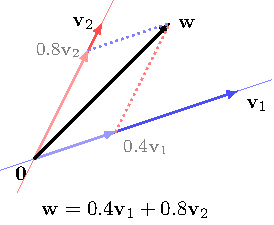
\includegraphics{figure/chapter01/basis-rep-a.pdf}
        \caption{}
        \label{fig:ch01-basis1}
    \end{subfigure}
    \begin{subfigure}[b]{0.28\textwidth}
        \centering
        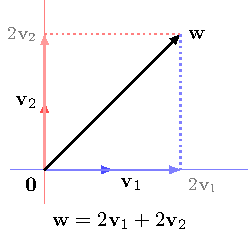
\includegraphics{figure/chapter01/basis-rep-b.pdf}
        \caption{}
        \label{fig:ch01-basis2}
    \end{subfigure}
    \begin{subfigure}[b]{0.40\textwidth}
        \centering
        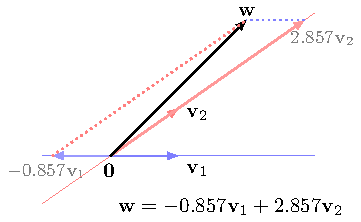
\includegraphics{figure/chapter01/basis-rep-c.pdf}
        \caption{}
        \label{fig:ch01-basis3}
    \end{subfigure}
    \caption{Representation of $\mf{w}$ in three different basis of $\mb{R}^2$. (a) and (c) are some arbitrary basis, while (b) is an orthonormal basis.}
\end{figure}

\subsection{Orthonormal basis}
Among the infinite number of basis for a vector space, there is a special class of basis called the \textit{orthonormal basis}. Let $V = \lc \mf{v}_1, \mf{v}_2, \cdots \mf{v}_n\rc$, then for an orthonormal basis, the following properties hold:
\begin{equation}
    \mf{v}_i^\top\mf{v}_j = \begin{cases} 1, & i = j \\ 0, & i \neq j \end{cases}
\end{equation}
This means that all basis vectors have unit 2-norm and are orthogonal to each other. We will come across orthonormal basis often in this course, and for a good reason. An orthonormal basis is easy to work with, and it's easy to compute the representation of a vector in an orthonormal basis. Let $V$ be an orthonormal basis for $\mb{R}^n$, and let $\mf{w} \in \mb{R}^n$ with the following representation,
\[ \mf{w} = \sum_{i=1}^n \alpha_i \mf{v}_i \]
Then, the coefficients $\alpha_i$ can be computed as the following:
\[ \mf{v}_j^\top\mf{w} =  \sum_{i=1}^n \alpha_i \mf{v}_j^\top\mf{v}_i = \alpha_j, \,\,\, \text{because } \mf{v}_i^\top\mf{v}_j = \begin{cases} 1, & i = j \\ 0, & i \neq j \end{cases} \]

A special orthonormal basis for the $\mb{R}^n$ is the \textit{standard basis} $\lc \mf{e}_1, \mf{e}_2 \cdots \mf{e}_n\rc$.

\section{Dimension of a vector space}
Although there can be an infinite number of basis for a vector space -- they all have the same number of elements or basis vectors. This number is called the \textit{dimension} of the vector space that they span. This is also sometimes called the 
\textit{degrees of freedom} of the vector space. We represent the dimension of a vector space $V$ as $\text{dim}\pp{V}$, e.g. $\text{dim}\pp{\mb{R}^n} = n$.

The dimension of a vector space also tells us the maximum number of linearly independent vectors we can choose from that vector space. For instance, in $\mb{R}^n$ we can only choose $n$ vectors that can form a linearly independent set. If we already have a linearly independent set with $n$ elements, then adding even one more vector (any vector) to the set will make it linearly dependent. Proper subspaces of a vector space will have dimensions less than the vector space itself.

\begin{boxedstuff}
    \begin{example}
        The dimension of $\mb{R}^n$ is $n$. The following are subspaces of $\mb{R}^n$ and their dimensions. Consider the set $V = \lc \mf{v}_1\rc$ with $\mf{v}_1 \neq \mf{0}$.
        \begin{itemize}
            \item $\text{dim}\pp{\text{span}\pp{V}} = 1$ 
            \item Now, let's add another vector $\mf{v}_2$ to $V$ to get $V_1 = \lc \mf{v}_1, \mf{v}_2 \rc$ which is still linearly independent, then
            \[ \text{dim}\pp{\text{span}\pp{V_1}} = 2 \]
            \item Let's now add the vector $\mf{v}_1 - \mf{v}_2$ to $V_1$ to get $V_2 = \lc \mf{v}_1, \mf{v}_2, \mf{v}_1 - \mf{v}_2 \rc$, then
            \[ \text{dim}\pp{\text{span}\pp{V_2}} = 2 \] \textcolor{red}{Why?}
            \item Consider the $V_k = \lc \mf{v}_1, \mf{v}_2, \cdots \mf{v}_k \rc$ which is linearly independent.
            \[ \text{dim}\pp{\text{span}\pp{V_k}} = ? \] \textcolor{red}{Can you find out the answer and explain?}
        \end{itemize}
    \end{example}
\end{boxedstuff}

\section{Linear functions}\label{sec:ch01-lin-func}
We will conclude this chapter with a brief introduction to linear functions. A function $f: \mb{R}^n \to \mb{R}$ is said to be linear if it satisfies the following property $\forall \mf{x}, \mf{y} \in \mb{R}^n$ and $\forall \alpha, \beta \in \mb{R}$:
\begin{equation}
    f\pp{\alpha \mf{x} + \beta \mf{y}} = \alpha f\pp{\mf{x}} + \beta f\pp{\mf{y}}
    \label{eq:linear-func-superpos}
\end{equation}
This means that $f\pp{\mf{0}} = 0$ for all linear functions. if a function does not satisfy this property, then it is not linear.

The standard inner product $\mf{w}^\top\mf{x}$ with a fixed  vector $\mf{w}$ is a linear function of $\mf{x}$,
\[ f\pp{\mf{x}} = \mf{w}^\top \mf{x} = w_1x_1 + w_2x_2 + \cdots + w_nx_n \]

An interesting fact about linear functions is that every possible $f: \mb{R}^n \to \mb{R}$ can be presented as an inner product operation with a fixed vector $\mf{w} \in \mb{R}^n$. This means the following: if $f$ is a linear function $\mb{R}^n$ to $\mb{R}$, then there exists a vector $\mf{w} \in \mb{R}^n$ such that $f\pp{\mf{x}} = \mf{w}^\top\mf{x}, \forall \mf{x} \in \mb{R}^n$. This might seem like a strange fact at first. Let's now look at how we could find the vector $\mf{w}$ if the function $f$ is linear. This is very simple. We first compute the value of the function for the $n$ unit vectors of $\mb{R}^n$, i.e. $f\pp{\mf{e}_1}, f\pp{\mf{e}_2}, \cdots f\pp{\mf{e}_n}$. Then, the vector $\mf{w}$ is simply the vector of these values, i.e. $\mf{w} = \bmxc f\pp{\mf{e}_1} \\ f\pp{\mf{e}_2} \\ \vdots \\ f\pp{\mf{e}_n} \emx = \bmxc w_1 \\ w_2 \\ \vdots \\ w_n \emx$. For any given vector $\mf{x}$, let the representation of $\mf{x}$ in the standard basis be $\mf{x} = \bmxc x_1 \\x_2 \\ \vdots \\ x_n\emx$; this simply means that $\mf{x} = \sum_{i=1}^n x_i\mf{e}_i$.
\[ 
\begin{split}
    f\pp{\mf{x}} = f\pp{\sum_{i=1}^nx_i\mf{e}_i} = \sum_{i=1}^nx_if\pp{\mf{e}_i} = \sum_{i=1}^nx_iw_i = \mf{w}^\top\mf{x}
\end{split}
\]

Here is another interesting consequence of linearity. If we know the value of a linear function for a set of vectors $X = \lc \mf{x}_1, \mf{x}_2, \cdots \mf{x}_k \rc$, then know the output of the function for the set $\text{span}\pp{X}$. Can you think of why it is so?

\section{Applications}
\secsum{
    The concepts convered in this chapter are enough to understand the following important and useful applications:
    \begin{itemize}
        \item k-nearest neighbors (k-NN) classification/regression algorithm
        \item k-means clustering algorithm
    \end{itemize}
}

We will now look at two applications in data analysis based on the concepts we have discussed in this chapter. We will present the bare-bones version of two commonly used algorithms in data analysis -- the k-nearest neighbors (k-NN) classification algorithm and the k-means clustering algorithm. Numerous variations and improvements of these algorithms exist, which are beyond the scope of this course.

\subsection{k-nearest neighbors (k-NN) classification and regression algorithms}
The k-NN algorithm is a simple and intuitive algorithm for classification and regression problems. But before that, what are classification and regression problems? Both of them are problems where one is interested in finding a function or a map from a set of features (or inputs) to a target value. The features are often in the form of $n$-vectors, and the target value is a scalar value. Classification and regression problems differ in the nature of the target value. In a classification problem, the target value is a class label (from a set of finite values), while in a regression problem, the target value is a real-valued number (from an interval on the real line).

\begin{boxedstuff}
    \vspace{4mm}
    \noindent{\large \textbf{Examples of classification problems}}
    \hrule
    \begin{example}
        \textbf{Disease diagnosis}. We are often interested in knowing whether or not a patient presenting with a set of symptoms at the hospital has a particular disease, based on clinical symptoms, and clinical lab tests. This is a typical example of a classification problem encountered in medicine. Given a set of features of a patient, the goal of the classifier is to determine whether the patient has a particular disease or not.
        \begin{itemize}
            \item \textbf{Inputs}: Set of demographic data, clinical tests, imaging data, etc.
            \item \textbf{Output}: Disease label (e.g., positive, negative, 0: no disease/1: disease, etc.)
        \end{itemize}
    \end{example}
    \begin{example}
        \textbf{Treatment prognosis}: Let's assume there is a treatment that can be used for curing a particular disease. This treatment works well on a group of patients who recover fully after the treatment, while some only recover partially, and the rest do not recover at all. Given a patient with this disease, the goal of the treatment prognosis classifier is to predict the effectiveness of the treatment for the patient. This classifier would take the features of the patient as input and predict the effectiveness of the treatment as one of three possible labels -- \textit{full recovery}, \textit{partial recovery} or \textit{no recovery}.
        \begin{itemize}
            \item \textbf{Inputs}: Set of demographic data, clinical tests, imaging data, severity of the disease, etc.
            \item \textbf{Output}: Recovery label (e.g., full recovery, partial recovery, or no recovery)
        \end{itemize}
    \end{example}
    \begin{example}
        \textbf{Spam email detection}: This is a classifier that we see in action on a daily basis. Our email managers/service providers automatically send certain emails to the spam folder to weed out the useless emails from the useful ones. Given an email, the goal of such a classifier is to determine whether the email is spam or not.
        \begin{itemize}
            \item \textbf{Inputs}: Features extracted from the email content, sender, subject, etc.
            \item \textbf{Output}: Spam label (e.g., spam, not spam)
        \end{itemize}
    \end{example}
    \begin{example}
        \textbf{Handwritten digit recognition}: Given an image of a handwritten digit, the classifier here needs to determine the corresponding digit of the image.
        \begin{itemize}
            \item \textbf{Inputs}: Image features extracted from the image of a handwritten digit.
            \item \textbf{Output}: Digit label (e.g., 0, 1, 2, ..., 9)
        \end{itemize}
    \end{example}

    \vspace{4mm}
    \noindent{\large \textbf{Examples of regression problems}}
    \hrule
    \begin{example}
        \textbf{Growth prediction}: We are interested in knowing the effect of the addition of protein supplements to the daily diet of children over a period of three months. The goal here is to develop a model that can predict the increase in height of the children after six months given a certain level of protein supplement in their diet.
        \begin{itemize}
            \item \textbf{Inputs}: Demographic details and amount of protein supplement in the diet.
            \item \textbf{Output}: Increase in child's height after six months.
        \end{itemize}
    \end{example}
    \begin{example}
        \textbf{Clinical score estimation}: There are clinical tests that are considered the gold standard for knowing the health status of a patient. These gold standard tests are often time-consuming, expensive, and difficult to administer on a regular basis. Thus, we are often interested in estimating the outcome of this gold standard test using other clinically relevant variables that are easily measured.
        \begin{itemize}
            \item \textbf{Inputs}: A set of clinically relevant parameters that are easy to measure.
            \item \textbf{Output}: Estimate of the value of the gold standard test.
        \end{itemize}
    \end{example}
\end{boxedstuff}

\subsubsection{k-NN classification algorithm}
The k-NN classifier is a very simple and intuitive algorithm. Let's assume that we have a dataset with $N$ data points/samples $\lp \mf{x}_i, y_i\rp, \,\, 1 \leq i \leq N$, where $\mf{x}_i$ is the vector of features, and $y_i$ is the know label for the $i^{th}$ sample. The feature vector is an element from $\mb{R}^n$, i.e. $\mf{x}_i \in \mb{R}^n$. The labels are taken on values from a finite set with $L$ distinct labels, $y_i \in \lc 1, 2, \ldots, L\rc$. We would like to use this available dataset, which will often be called the \textit{training dataset}, to learn to correctly classify new samples that we may encounter in the future, where we have the feature vector $\mf{x}_{new}$ but we do not know the corresponding label $y_{new}$; we want a prediction of the label from the k-NN algorithm. 

Although the k-NN algorithm is called a \textit{supervised learning} algorithm, there is really no learning in this algorithm. The algorithm keeps the entire training dataset in its memory and assigns the label to a new feature vector to be the label of the most similar feature vectors from the training dataset. The similarity can be measured through a multitude of ways, but the most common way is to use the Euclidean distance between the feature vectors. The only (hyper)parameter required for the k-NN algorithm is the value of $k$, which is the number of nearest neighbors to consider. The label of the new feature vector is assigned by taking a vote from the $k$-nearest neighbors. The label with the highest number of votes is assigned to the new feature vector. The outline of the k-NN algorithm is given below in Algorithm~\ref{alg:ch01-knn-class}.

\begin{boxedstuff}
\begin{algorithm}[H]
    \SetAlgoLined
    \KwData{Training data $\lp \mf{x}_i, y_i \rp \,\, 1 \leq i \leq N$; test point $\mf{x}_{new}$; number of neighbors $k$.}
    \KwResult{Predicted label for test point $\mf{x}_{new}$.}
    
    \BlankLine
    \ForEach{$\mf{x}_j$ in $\lp \mf{x}_i \rp_{i=1}^N$} {
        Compute the distance $d(\mf{x}_j, \mf{x}_{new})$ between $\mf{x}_j$ and $\mf{x}_{new}$\;
    }
    
    Sort the training instances/samples $\lp \mf{x}_i, y_i\rp$ by distance in ascending order\;
    Select the $k$ closest samples to $\mf{x}_{new}$; let $\mc{K}$ be the set of indices between 1 to $N$ corresponding to these $k$ closest samples\; let $Y_{\mc{K}}$ be the set of labels of these $k$ closest samples\;
    \BlankLine
    \ForEach{label in $Y_\mc{K}$}{
        Compute the frequency of each label\;
    }
    
    Return the label with the highest frequency\;
    \caption{k-Nearest Neighbors (k-NN) Algorithm}
    \label{alg:ch01-knn-class}
\end{algorithm}
\end{boxedstuff}

This is depicted in Figure~\ref{fig:ch01-knn-demo}, which shows the example of a 3-class classification problem. The three classes are shown in different colors. The $k=5$ nearest neighbors of three test points are shown. The label of the test point is assigned based on the majority vote of the $k$ nearest neighbors; whenever there is a tie, a tie-breaking rule is applied to choose the label of the test point. Although simple and intuitive, the k-NN is a computationally expensive algorithm, especially when the number of samples in the training dataset is large. The advantage, however, is that there is no training process required, and there is only a hyperparameter to choose from.

\begin{figure}
    \centering
    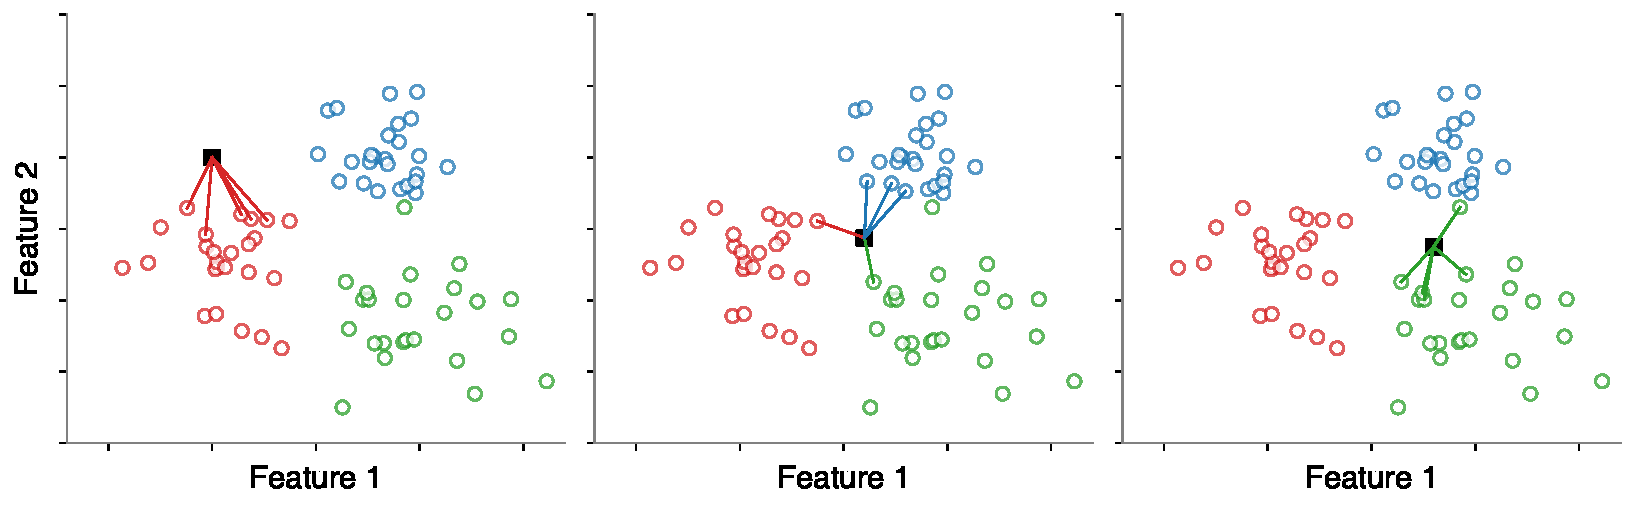
\includegraphics[width=0.8\textwidth]{figure/chapter01/knn.pdf}
    \caption{Demonstration of the k-NN classification algorithm. There are three classes of labels, which are shown in different colors. Three test points (black filled square) are considered in the three plots shown in this figure. For each point, the $k=5$ nearest neighbours are depicted through lines joining the test point with the nearest neighbours. The colors of the line also indicate the class of that neighbour.}
    \label{fig:ch01-knn-demo}
\end{figure}

\subsubsection{k-NN regression algorithm}
The k-NN regression algorithm uses the same principle as the k-NN classification algorithm. The only difference is that the output of the algorithm is the average of the $y_i$ of the $k$ nearest neighbors. This algorithm is detailed in Algorithm~\ref{alg:ch01-knn-reg}.

\begin{boxedstuff}
    \begin{algorithm}[H]
    \SetAlgoLined
    \KwData{Training data $\lc \lp \mf{x}i, y_i \rp \rc{i=1}^N$; test point $\mf{x}{new}$; number of neighbors $k$.}
    \KwResult{Predicted value for test point $\mf{x}{new}$.}    
    \BlankLine
    \ForEach{$\mf{x}_j$ in $\lc \mf{x}_i \rc_{i=1}^N$}{
        Compute the distance $d(\mf{x}_j, \mf{x}_{new})$ between $\mf{x}_j$ and $\mf{x}_{new}$\;
    }
    Sort the training instances/samples $\lp \mf{x}_i, y_i \rp$ by distance in ascending order\;
    Select the $k$ closest samples to $\mf{x}_{new}$; let $\mc{K}$ be the set of indices between 1 to $N$ corresponding to these $k$ closest samples\; let $Y_{\mc{K}}$ be the set of values of these $k$ closest samples\;
    \BlankLine
    Compute the average of the values in $Y_{\mc{K}}$\;
    
    Return the computed average as the predicted value\;
    \caption{k-Nearest Neighbors (k-NN) Regression Algorithm}
    \label{alg:ch01-knn-reg}
    \end{algorithm}
\end{boxedstuff}

\begin{figure}
    \centering
    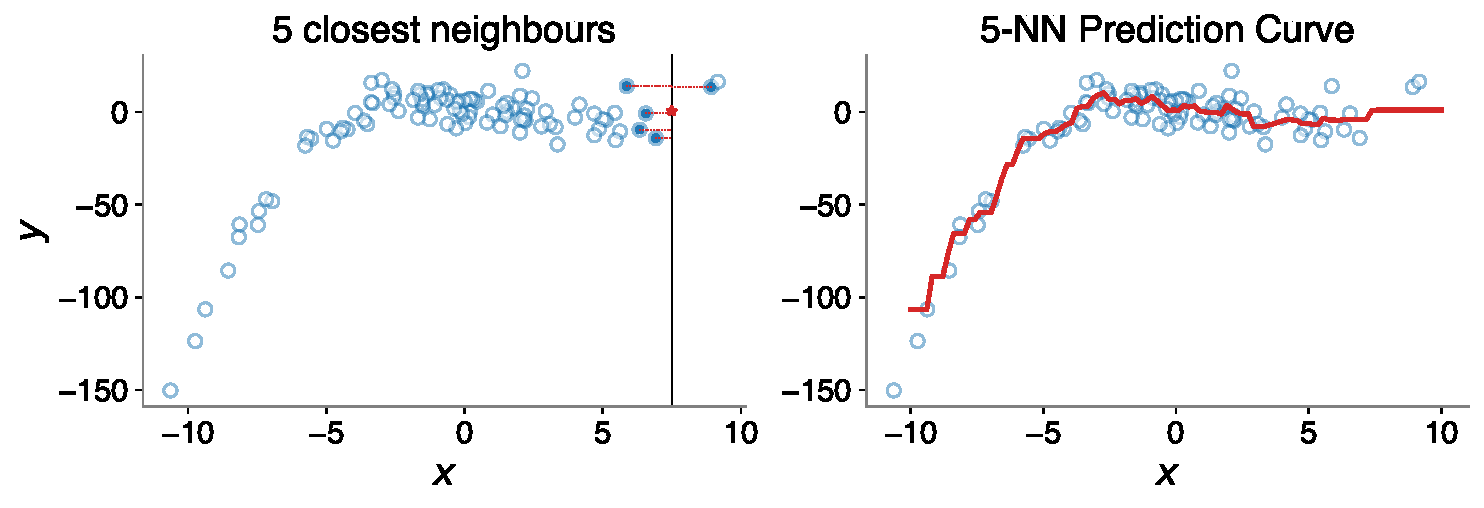
\includegraphics[width=0.85\textwidth]{figure/chapter01/knn-reg.pdf}
    \caption{Demonstration of the k-NN regression algorithm. In this example, $\mf{x} \in \mb{R}$. The left plot demonstrates the algorithm, where the vertical black line is the $\mf{x}_{new}$, the filled blue circles are the 5 closest neighbours. The red star along the black line is the predicted value for $\mf{x}_{new}$. The right plot shows the $5$-NN prediction curve for the given data in red.}
    \label{fig:ch01-knn-reg-demo}
\end{figure}

\subsection{k-mean clustering algorithm}
The $k$-mean is a popular clustering algorithm, which, unlike the k-NN algorithms, is an \textit{unsupervised learning} algorithm. In a \textit{supervised learning} algorithm, we have a dataset that has an output label or numerical value of interest, which can be used to learn the association between the given features and the output label/numerical value. However, we will often come across datasets where there is no such pre-existing output label or numerical value or it is unknown. In such cases, we are simply interested in interesting patterns (clusters or groups) in the data; we need to mathematically define what we mean by ``interesting'' to find such patterns. The k-means algorithm lumps data points into $k$ clusters or groups, where the elements of the cluster/group are considered to be similar; remember the discussion on measuring similarity between vectors in Section~\ref{sec:ch01-similar-vecs}.

Let's assume that our dataset consists of $N$ samples, each of which is a feature vector, $\mf{x}_i \in \mb{R}^n, \, 1 \leq i \leq N$. We want to group the data points into $k$ clusters with $k < N$. Given the data points $\mf{x}_1 \ldots \mf{x}_N$, the k-means algorithm produces two outputs:
\begin{enumerate}
    \item \textbf{Cluster means}: A set of $k$ points $\mf{m}_j \in \mb{R}^n, \, 1 \leq j \leq k$ that are supposed to be representatives of the $k$ clusters identified. You can think of $\mf{m}_j$ to be a typical member of the $j^{th}$ cluster.
    \item \textbf{Cluster assignment}: Each data point $\mf{x}_i$ is given a cluster assignment $j$, such that $\mf{x}_i$ is closest to $\mf{m}_j$. This is an $N$-tuple of the form $\lp c_i \rp_{i=1}^N$, with $1 \leq c_i \leq k$. If $c_i = j$, then the data point $\mf{x}_i$ belongs to the $j^{th}$ cluster.
\end{enumerate}

\begin{figure}
    \centering
    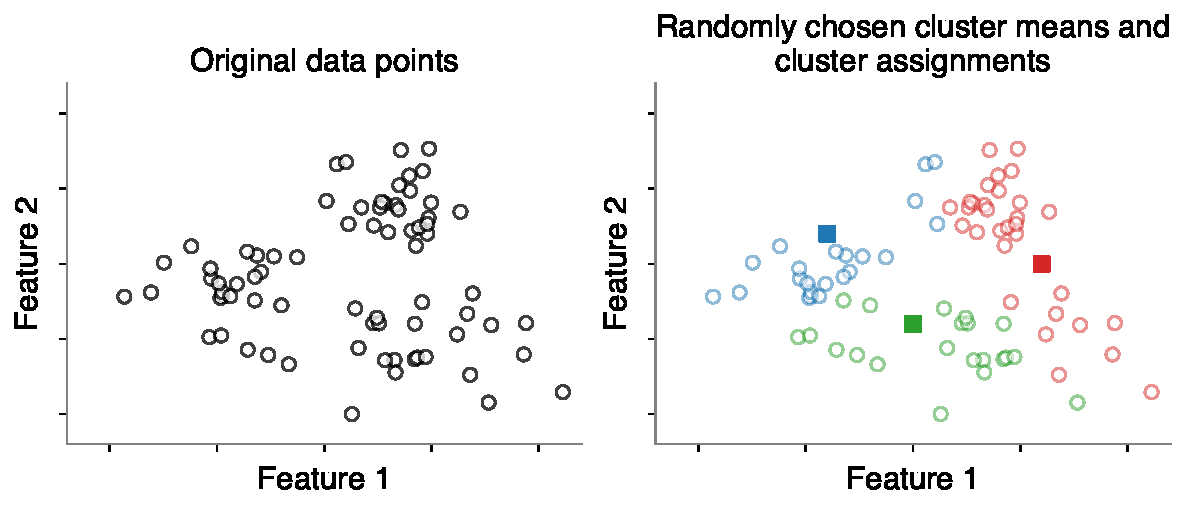
\includegraphics[width=0.67\textwidth]{figure/chapter01/kmeans-demo.pdf}
    \caption{The clustering problem tackled by the k-means algorithm. The lft plot shows  }
    \label{fig:ch01-kmeans-demo}
\end{figure}

This is demonstrated in Figure~\ref{fig:ch01-kmeans-demo}, where the left plot shows the dataset with $N$ samples, each belonging to $\mb{R}^2$. The right plot shows three randomly chosen cluster means $\mf{m}_1, \mf{m}_2, \mf{m}_3$ and the cluster assignment of the data points to the closest $\mf{m}_j$. The three cluster means are shown in different colors and the corresponding data points in those clusters are shown in the same color (but a lighter shade). The goal for the k-means algorithm is to find the optimal cluster means and the cluster assignment such that the spread of points within each cluster is minimized across all clusters. We can measure this spread as the following,
\begin{equation}
    J_{clust} = \frac{1}{N}\sum_{j=1}^k \sum_{i \in C_j} \lV \mf{x}_i - \mf{m}_j \rV_2^2
    \label{eq:ch01-kmeans-cost}
\end{equation}
where, $C_j = \lc i \, : \, 1 \leq i \leq N, \, c_i = j\rc$ is the set of indices of the data points that belong to the cluster $j$.

Minimizing $J_{clust}$ for a given dataset is a computationally intensive problem. Note that the cluster means and the cluster assignments both depend on each other, and optimally choosing both of them to minimize $J_{clust}$ is not easy. 

The k-means simplifies the computational problem because choosing the optimal cluster means for a fixed cluster assignment and choosing the optimal cluster assignment for fixed cluster means is easy to do. The k-mean algorithm optimizes the cluster means and cluster assignments while fixing the other and iterates these steps until the cluster means and cluster assignments converge. This algorithm is detailed in Algorithm~\ref{alg:ch01-kmeans}.

\begin{boxedstuff}
    \begin{algorithm}[H]
    \SetAlgoLined
    \KwData{Dataset $\mf{x}_1 \ldots \mf{x}_N$; number of cluster $k$ tp be identified.}
    \KwResult{A set of $k$ cluster means $\mf{m}_1, \dots, \mf{m}_k$ and a $N$-tuple of cluster assingments $\lp c_i \rp_{i=1}^N$.}    
    \BlankLine
    Choose a random set of $k$ cluster means $\mf{m}_1,\ldots,\mf{m}_k$\;

    \Repeat{until convergence}{
        \textbf{Update cluster assignment}: For the current means, find the best cluster assignment. $c_i = j$, such that $\lV \mf{x}_i - \mf{m}_j \rV_2 < \lV \mf{x}_i - \mf{m}_l\rV_2, \forall \,\, 1 \leq l \leq k, l \neq j$\;
        
        \textbf{Update cluster means}: For the new cluster assignment, find the best cluster means. $\mf{m}_j = \frac{1}{\lv C_j \rv}\sum_{i \in C_j}$, where $C_j$ is the set of indices of data points for the $j^{th}$ cluster and $\lv \cdot \rv$ is a function that returns the number of elements in a set\;
    }
    Return the cluster means $\mf{m}_1 \ldots \mf{m}_k$ and the cluster assignment $\lp c_i \rp_{i=1}^N$\;
    \caption{k-means Clustering Algorithm}
    \label{alg:ch01-kmeans}
    \end{algorithm}
\end{boxedstuff}


This is demonstrated in Figure~\ref{fig:ch01-kmeans-demo}. The top left plot shows the dataset with $N$ samples without any cluster assignment; all data points are colored black. The top right plot shows the first step in the iteration where the cluster means were chosen randomly; these are shown in different colored filled triangles. The corresponding optimal cluster assignment of points that are closest to each mean is also depicted in this plot.

\begin{figure}[h]
    \centering
    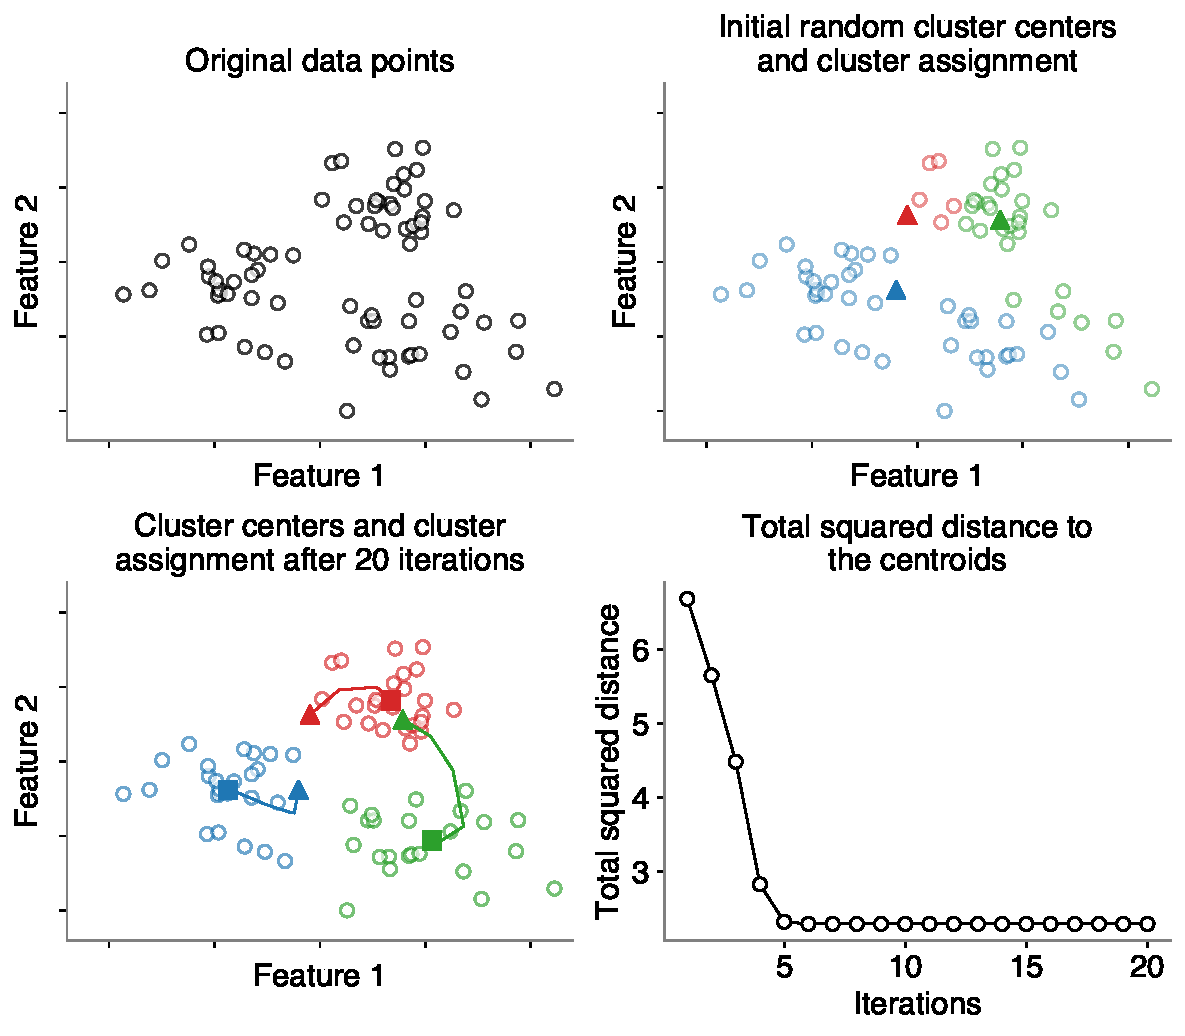
\includegraphics[width=0.67\textwidth]{figure/chapter01/kmeans-algo.pdf}
    \caption{The clustering problem tackled by the k-means algorithm. The left plot shows  }
    \label{fig:ch01-kmeans-algo}
\end{figure}

The bottom left plot shows the trajectory of the cluster means as the k-means algorithm iterates, repeating the process of updating the cluster means and cluster assignments. The two steps in of the $k$-means algorithm are guaranteed to reduce $J_{clust}$, and thus, with each iteration, the value of $J_{clust}$ for the current cluster means and cluster assignments will reduce. This is depicted in the bottom right plot, which shows the trend of $J_{clust}$ as a function of the iteration number.

\section{Exercise}
\vspace{-0.5cm}
\begin{center}
    \rule{\textwidth}{1pt}
\end{center}

\begin{enumerate}
    \item Is this set of vectors $\left\{\begin{bmatrix}2 \\ 1 \\ 1\end{bmatrix}, \begin{bmatrix}0 \\ 0\\ 0\end{bmatrix}, \begin{bmatrix}0 \\ 1 \\ 0\end{bmatrix}\right\}$ independent? Explain your answer.
    
    \item Show that the set $\lc \mf{0} \rc$, $\mf{0} \in \mb{R}^n$ a subspace of $\mb{R}^n$? This is called the trivial subspace of $\mb{R}^n$. What is the dimension of this subspace?
    
    \item Prove the following for $\mf{x}, \mf{y} \in \mathbb{R}^n$,
    \begin{enumerate}
        \item {\small \textbf{Triangle Inequality}}:
        \[ \left\lVert \mf{x} + \mf{y}\right\rVert \leq \left\lVert \mf{x}\right\rVert + \left\lVert \mf{y}\right\rVert \]
        \item {\small \textbf{Backward Triangle Inequality}}:
        \[ \left\lVert \mf{x} - \mf{y}\right\rVert  \geq \left\lvert \left\lVert \mf{x}\right\rVert - \left\lVert \mf{y}\right\rVert \right\rvert \]
        \item {\small \textbf{Parallelogram Identity}}:
        \[ \frac{1}{2} \left(\left\lVert \mf{x} + \mf{y}\right\rVert^2 + \left\lVert \mf{x} - \mf{y}\right\rVert^2 \right) = \left\lVert \mf{x}\right\rVert^2 + \left\lVert \mf{y}\right\rVert^2 \]
    \end{enumerate}

    \item Consider a set of vectors $\mf{x}, \mf{y} \in \mathbb{R}^n$. When is $\left\lVert \mf{x} - \mf{y} \right\rVert = \left\lVert \mf{x} + \mf{y}\right\rVert$? What can you say about the geometry of the vectors $\mf{x},\,\mf{y},\,\mf{x} - \mf{y}$ and $\mf{x} + \mf{y}$? 
    
    \item Find the $1$, $2$ and $\infty$ norms of the following vectors from $\mb{R}^3$:
    
    \begin{enumerate*}
        \item $\bmxc 1 \\ 0 \\ 1 \emx$
        \item $\bmxc 0 \\ 0 \\ 0 \emx$
        \item $\mf{e}_3$
        \item $\bmxc a \\ b \\ c \emx$
        \item $\mf{e}_1 - \mf{e}_2 + \mf{e}_3$
    \end{enumerate*}

    \item If $S_1, S_2 \subseteq V$ are subspaces of a vectors space $V$ then, is $S_1 \cap S_2$ a subspace? Is $S_1 \cup S_2$ a subspace? Explain your answers.
    
    \item Consider a vector $\mf{v} = \begin{bmatrix*}v_1 & v_2 & \cdots & v_n\end{bmatrix*}^\top$. Express the following in terms of the inner product between a constant vector $\mf{u}$ and the given vector $\mf{v}$, and in each case, specify the vector $\mf{u}$.
    \begin{enumerate}
        \item $\sum_{i=1}^n v_i$
        \item $\frac{1}{n}\sum_{i=1}^n v_i$
        \item $\frac{1}{5}\sum_{i=3}^5 v_i$
    \end{enumerate} 
    
    \item Which of the following are linear functions of $\left\{x_1, x_2, \ldots,x_n\right\}$?
    \begin{enumerate}
        \item $\min_i \left\{x_i\right\}_{i=1}^{n}$
        \item $\left(\sum_{i=1}^n x_i^2\right)^{1/2}$
        \item $x_6$
    \end{enumerate}

    \item Consider a linear function $f: \mathbb{R}^n \rightarrow \mathbb{R}$. Prove that every linear function of this form can be represented in the following form.
    \[ y = f\left(\mf{x}\right) = \mf{w}^\top\mf{x} = \sum_{i=1}^{n}w_ix_i, \quad \quad \mf{x}, \mf{w} \in \mathbb{R}^n \]

    \item An \textit{affine} function $f$ is defined as the sum of a linear function and a constant. It can in general, be represented in the form, 
    \[ y = f\left(\mf{x}\right) = \mf{w}^\top\mf{x} + \beta, \quad \quad \mf{x}, \mf{w} \in \mathbb{R}^n, \, \beta \in \mathbb{R} \]
    Prove that affine functions are not linear. Prove that any affine function can be represented in the form $\mf{w}^\top\mf{x} + \beta$.

    \item Consider a basis $B = \left\{\mf{b}_i\right\}_{i=1}^{n}$ of $\mb{R}^n$. Let the vectors $\mf{x}$ and $\mf{x}_b$ be the representations in the standard and $B$ basis, respectively. 
    \[ \mf{x} = \begin{bmatrix*}x_1\\x_2\\\vdots\\x_n\end{bmatrix*} = \sum_{i=1}^{n}x_i\mf{e}_i \,\,\,\,\, \text{and} \,\,\,\,\, \mf{x}_b =  \begin{bmatrix*}x_{b1}\\x_{b2}\\\vdots\\x_{bn}\end{bmatrix*} = \sum_{i=1}^{n}x_{bi}\mf{b}_i \]

    Evaluate the $\left\lVert \mf{x}\right\rVert_2^2$ and $\left\lVert \mf{x}_b\right\rVert_2^2$. Determine what happens to $\left\lVert \mf{x}_b\right\rVert_2^2$ under the following conditions on the basis vectors: \textbf{[Marks: 2]}
    \begin{enumerate}
        \item $\left\lVert \mf{b}_i\right\rVert = 1, \forall i$
        \item $\left\lVert \mf{b}_i^\top\mf{b}_j\right\rVert = \begin{cases}
        1 & i = j\\
        0 & i \neq j
        \end{cases}$
    \end{enumerate}

    \item \textcolor{blue}{\textbf{[Programming]}} Let's build a simple classifier using the concepts you've learned in this chapter. We will pretend that we are doing this to classify or detect the presence or absence of a disease called - \textit{vector space sickness}. We wish to diagnose using two clinical tests - (1) \textit{Subspace assay} and (2) \textit{Basis balance scale}. Both these serious clinical tests generate numerical outcomes that can take on any real number value.
    
    The department has been conducting a large-scale clinical study for the last 5-6 years, collecting data from participants from different backgrounds, with and without vector space sickness, by administering the subspace assay and the basis balance test. The data from this study is stored as a CSV file with four columns: (a) \textcolor{blue}{\texttt{subjectno}} -- subject numbers, (b) \textcolor{blue}{\texttt{x1}} --  value of the subspace assay test, (c) \textcolor{blue}{\texttt{x2}} -- value of the basis balance scale, and (d) \textcolor{blue}{\texttt{vss}} -- presence (1) or absence (0) of the vector space sickness condition. Each row of this CSV file corresponds to an individual subject who participated in the study. Your goal here is to look at the data from this experiment and propose a classifier to determine if a person has vector space sickness if we are given their scores on the subspace assay and the basis balance scale clinical tests. A group of Master's students participated in the study. Unfortunately, almost half of these students were diagnosed with vector space sickness. This data is stored in \textcolor{blue}{\texttt{expt1.csv}}. Read this data and make a scatter plot in 2D (\texttt{x1} versus \texttt{x2}) with the data points for participants with vector space sickness in blue and the one without in red. Look at the data and propose how you could use the measurements \texttt{x1} and \texttt{x2} to distinguish between participants from the two groups. Implement the classifier you've proposed and find out how well it performs in correctly classifying the two groups.

    \item \textcolor{blue}{\textbf{[Programming]}} Consider a set of measurements made from adult male subjects, where their height, weight, and BMI (body mass index) were recorded and stored as vectors of length three; the first element is the height in $cm$, second is the weight in $Kg$, and the last is the BMI. Consider the following four subjects,
    \[ \mf{s}_1 =  \begin{bmatrix*}[r]167\\102\\36.6\end{bmatrix*}; \,\,
    \mf{s}_2 =  \begin{bmatrix*}[r]180\\87\\26.9\end{bmatrix*} \,\, \mf{s}_3 =  \begin{bmatrix*}[r]177\\78\\24.9\end{bmatrix*}; \,\,
    \mf{s}_4 =  \begin{bmatrix*}[r]152\\76\\32.9\end{bmatrix*} \]

    You can use the distance between these vectors $\left\lVert \mf{s}_i - \mf{s}_j\right\rVert_2$ as a measure of the similarity between the four subjects. Generate a $4 \times 4$ table comparing the distance of each subject with respect to another subject; the diagonal elements of this table will be zero, and it will be symmetric about the main diagonal. 

    (a) Based on this table, how do the different subjects compare to each other?

    (b) How do the similarities change if the height had been measured in $m$ instead of $cm$? Can you explain this difference?

    (c) Consider the weighted norm presented in one of the earlier problems.  
    \[ \left\lVert x \right\rVert_\mf{w} = \left(w_1 x_1^2 + w_2 x_2^2 + \cdots + w_n x_n^2\right)^{\frac{1}{2}} \]
    Will this fix the problem? What would be a good choice for $\mf{w}$ to address the problems with comparing distance between vectors due to unit change?

    (d) Can the angle between two vectors be used as a measure of similarity between vectors? Does this suffer from the problem of the 2-norm $\left\lVert \cdot \right\rVert_2$?
\end{enumerate}


